%! TEX root = ../../main_netxpto.tex
\clearpage

\subsection{Experimental Setup}
	The setup shown in Figure~\ref{fig:experimental_mqam_setup} was used to obtain
	experimental results to compare with the theory and validate the simulation. The
	list of devices used for the setup is available in Table~\ref{tab:mqamdevices}.
	Tables~\ref{tab:rxParamsNew} to~\ref{tab:edfaParams} show the devices'
	specifications.
	\begin{figure}[H]
		\centering
		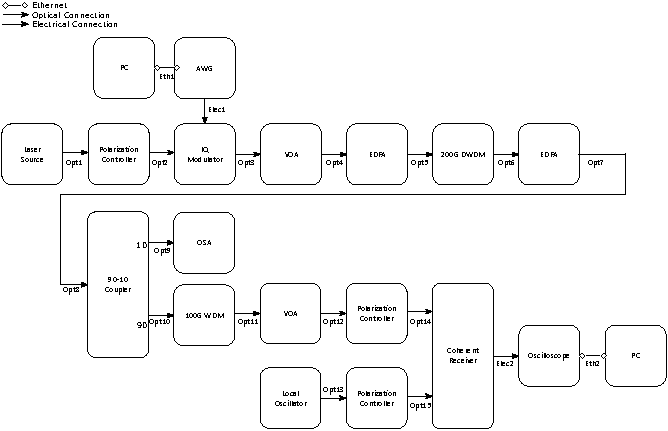
\includegraphics[width=\textwidth]{./sdf/m_qam_system/figures/experimental/experimentalSetup/mqamExperimental.pdf}
		\caption{Experimental setup}
		\label{fig:experimental_mqam_setup}
	\end{figure}
	\begin{figure}[H]
		\centering
		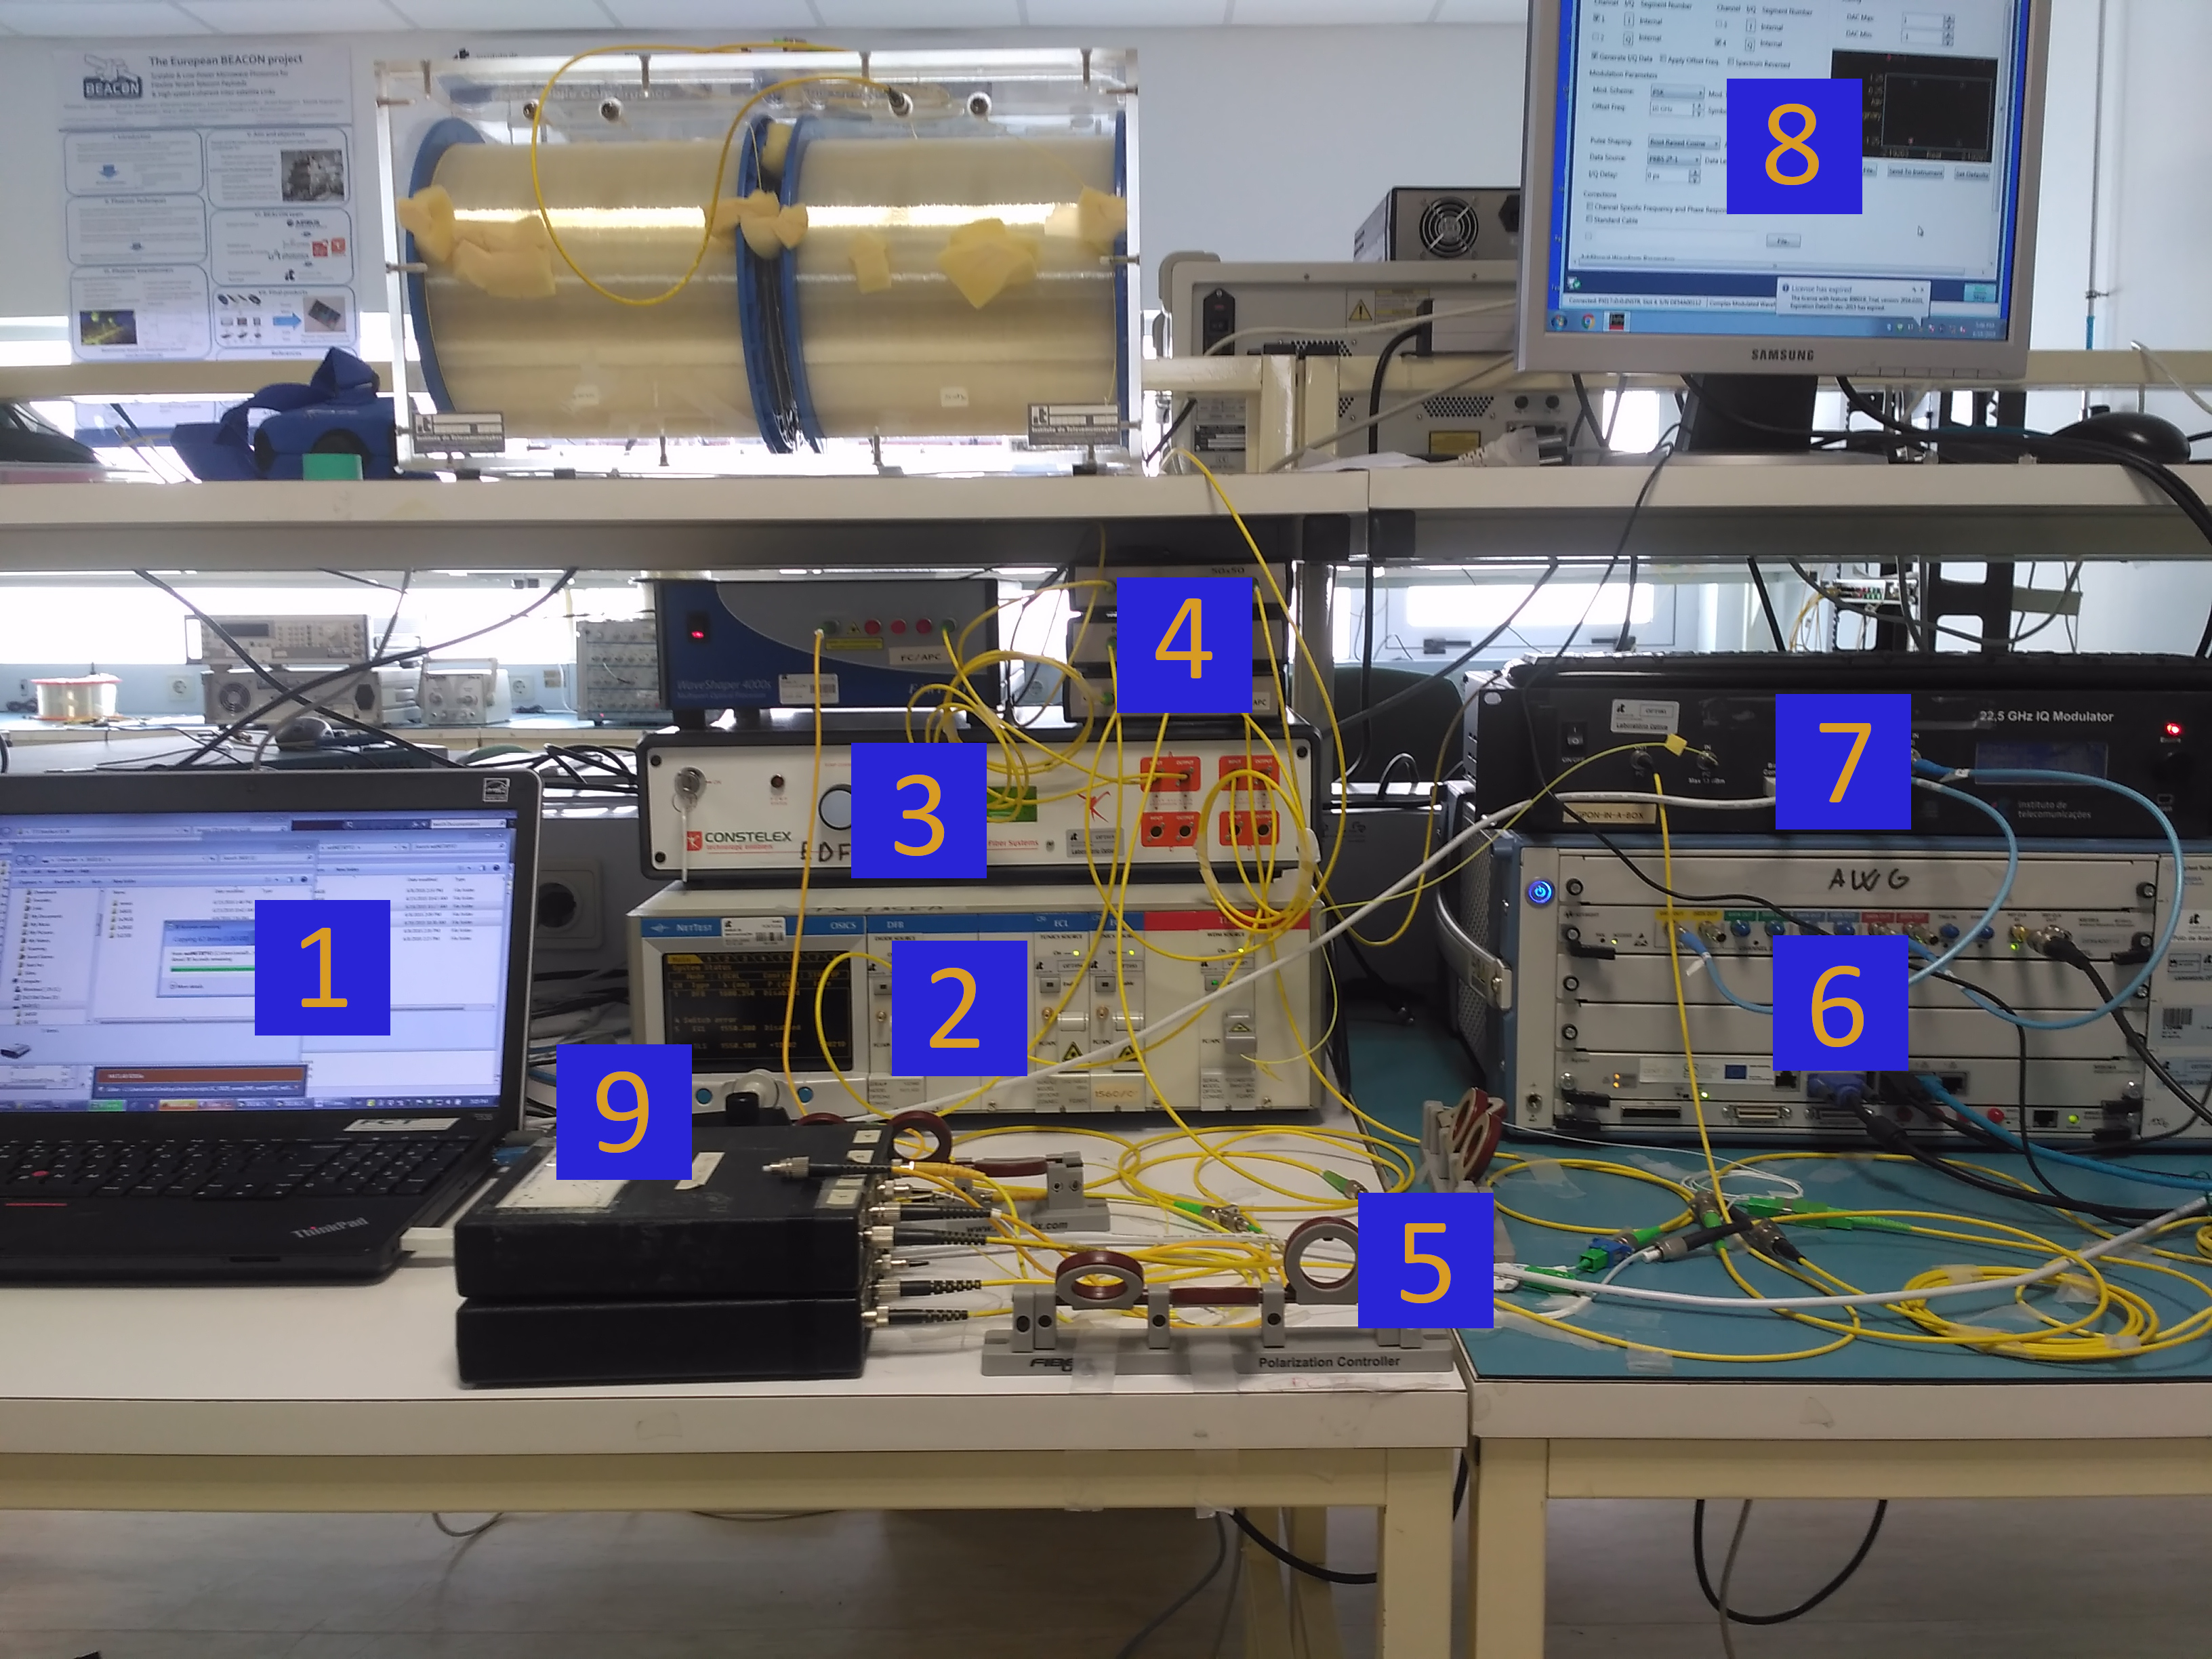
\includegraphics[width=0.65\textwidth]{./sdf/m_qam_system/figures/experimental/experimentalSetup/setupLeft.jpg}
		\caption{Photo of the experimental setup. 1-Computer; 2-TX Laser source; 3-EDFA; 4-Couplers and filters;
		5-Polarization controllers; 6-AWG; 7-IQ Modulator; 8-AWG monitor; 9-USB controlled variable optical attenuator.}
		\label{fig:experimental_mqam_setup_photo_left}
	\end{figure}
	\begin{figure}[H]
		\centering
		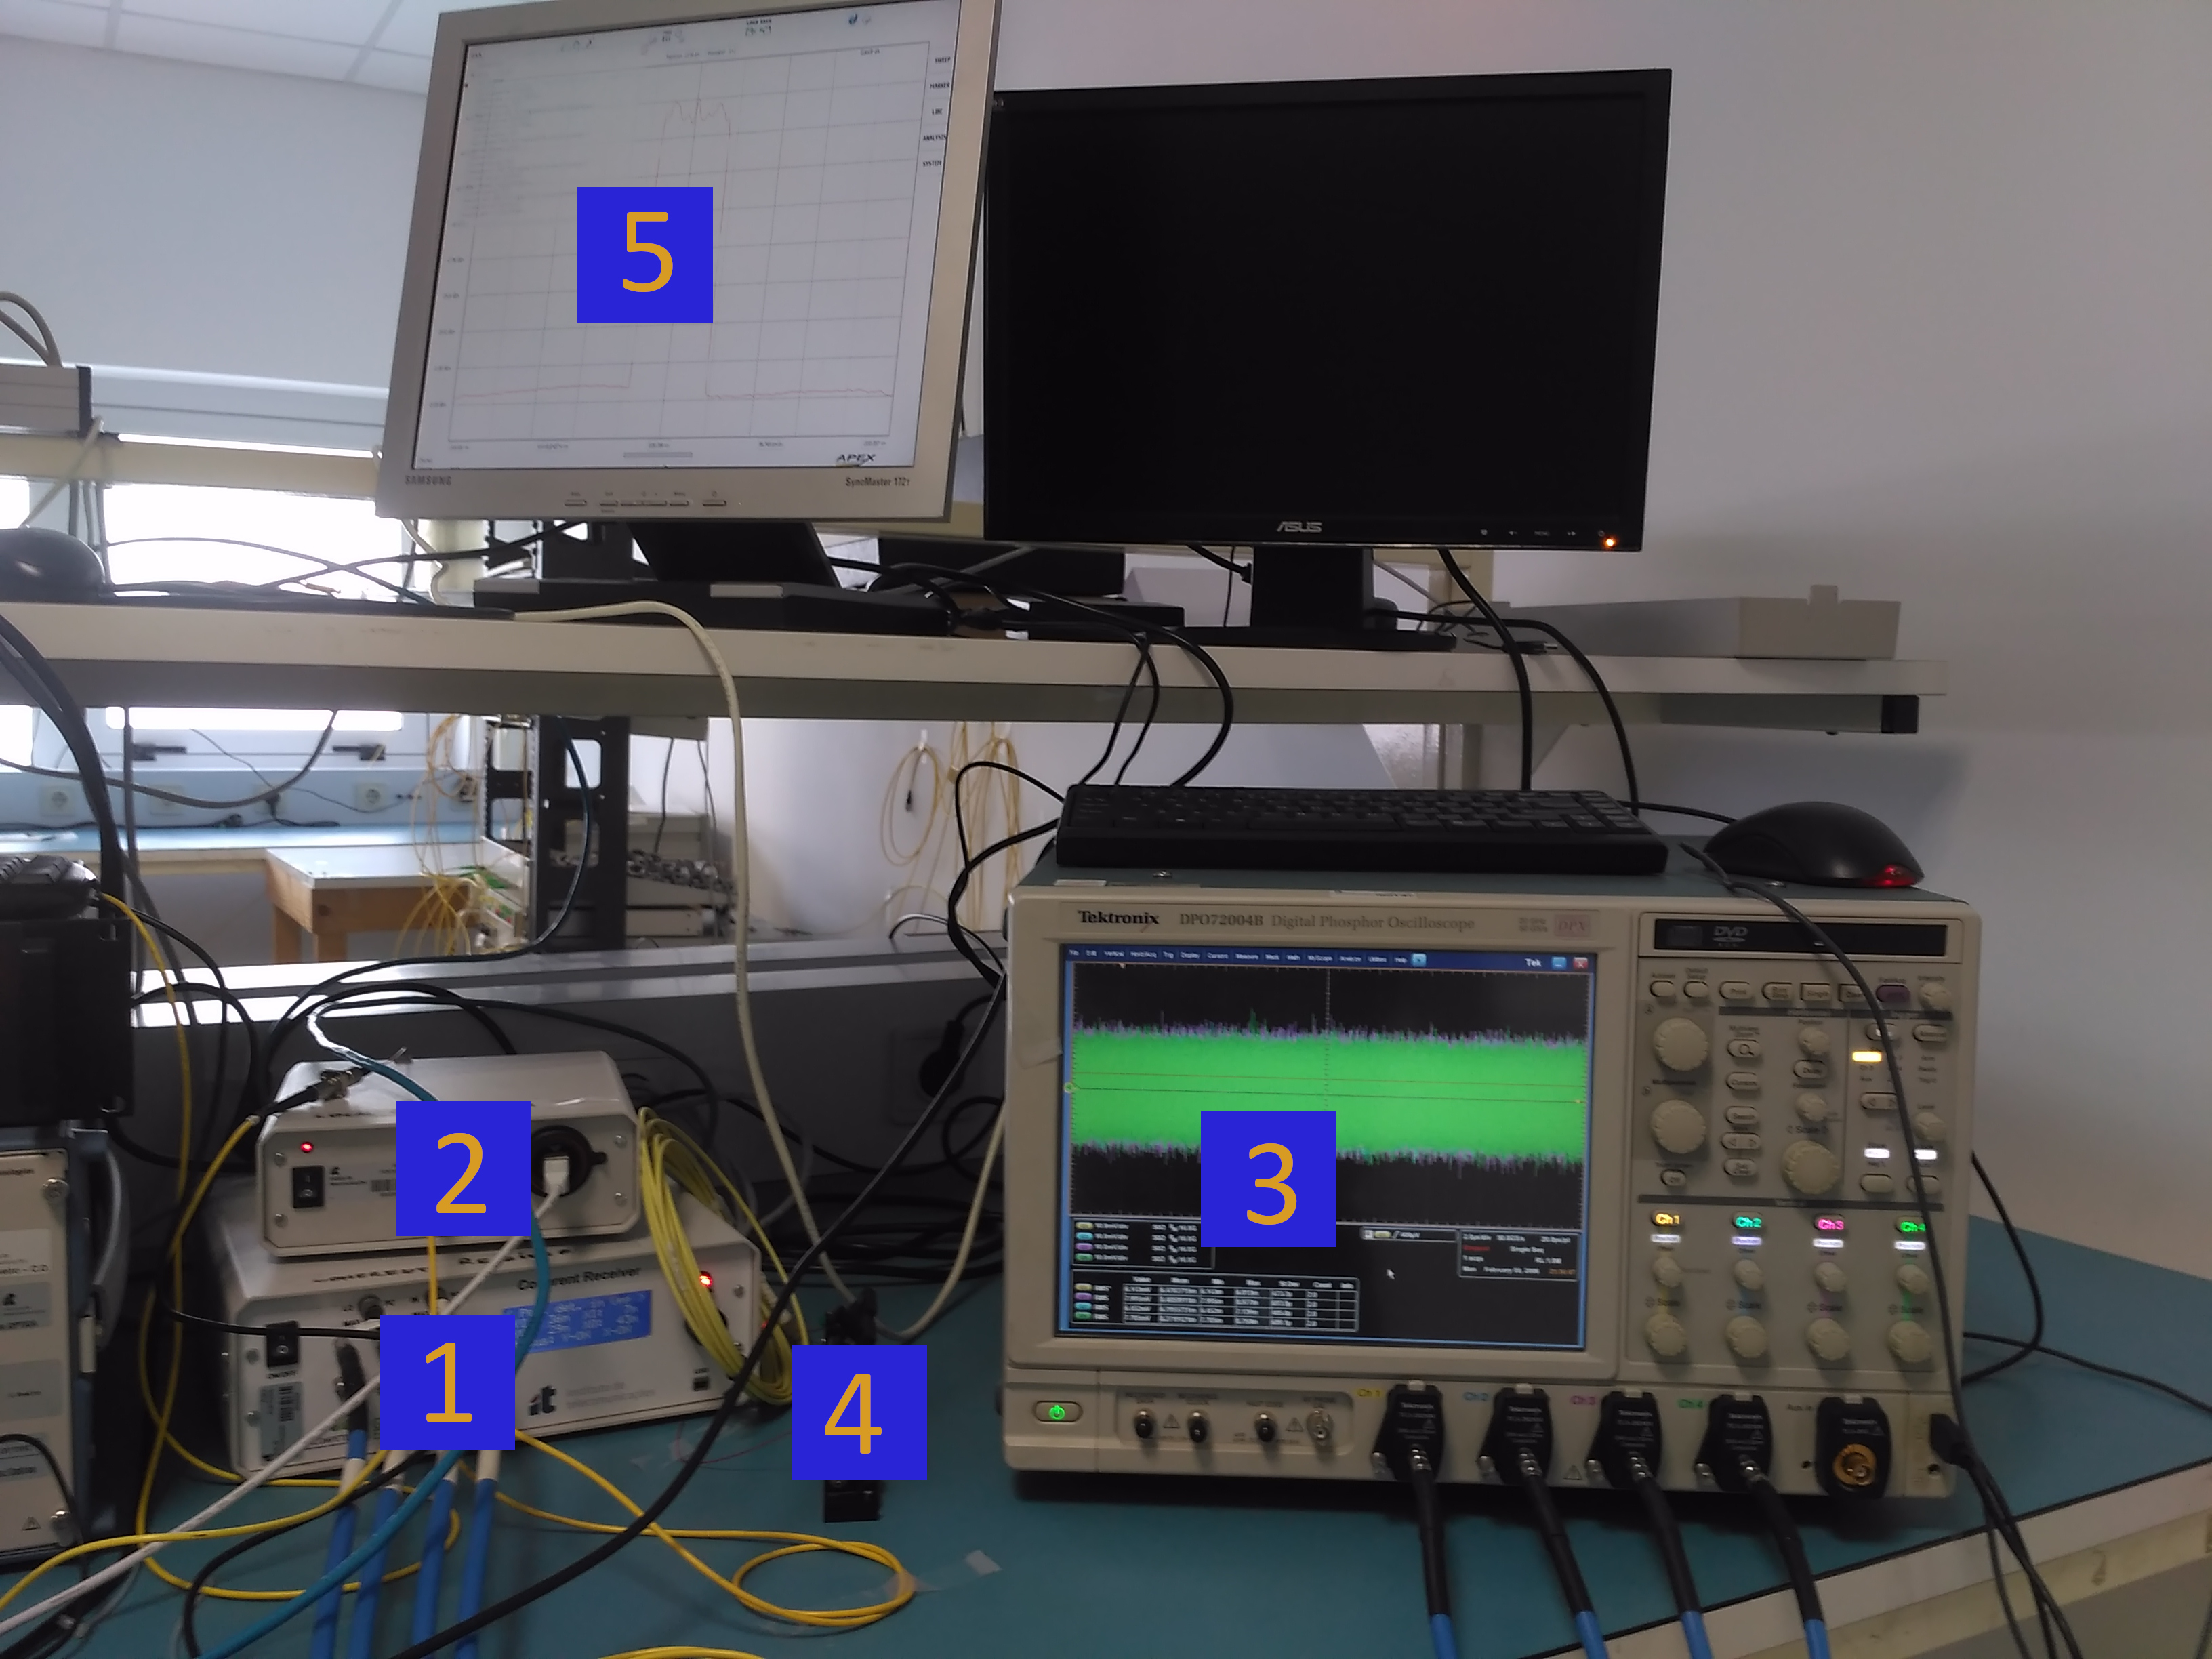
\includegraphics[width=0.65\textwidth]{./sdf/m_qam_system/figures/experimental/experimentalSetup/setupRight.jpg}
		\caption{Photo of the experimental setup. 1-Coherent Receiver; 2-Local Oscillator laser source; 3-Oscilloscope; 4-Polarization controller; 5-OSA monitor.}
		\label{fig:experimental_mqam_setup_photo_right}
	\end{figure}
	\begin{table}[H]
		\centering
		\begin{tabulary}{1.0\textwidth}{|L|L|l|}
			\hline
			\textbf{Device}		& \textbf{Model}					& \textbf{Description}\\\hline
			Laser Source		& Yenista OSICS Band C/AG TLS Laser			& Optical laser source for modulate the signal \\\hline
			IQ Modulator		& 22.5GHz IQ Modulator with automatic Bias Controller	& \\\hline
			AWG			& Keysight M8195A					& \\\hline
			VOA			&							& USB-Controlled Variable Optical Attenuator \\\hline
			EDFA			& Constelex Hydra-C-17-17 EDFA				& \\\hline
			200G DWDM		&							& \\\hline
			EDFA			& Constelex Hydra-C-17-17 EDFA				& \\\hline
			90/10 Coupler		&							& \\\hline
			OSA			& Apex Technologies AP-2043B				& \\\hline
			100G WDM		&							& \\\hline
			VOA			&							& \\\hline
			Local Oscillator	& Emcore CRTND3U02D ECL Laser				& \\\hline
			Coherent Receiver	& Picometrix CR-100D					& \\\hline
			Oscilloscope		& Tektronix DP720004B				& \\\hline
		\end{tabulary}
		\caption{Devices in experimental setup.~\label{tab:mqamdevices}}
	\end{table}
	Tables~\ref{tab:rxParamsNew} to~\ref{tab:edfaParams} list the relevant
	specifications for the devices used in the experimental setup.

	\subsubsection{Device Specifications}
	\begin{table}[H]
		\centering
		\begin{tabulary}{1.0\textwidth}{|L|l|}
			\hline
			\multicolumn{2}{|c|}{\textbf{Tektronix DP720004B Oscilloscope, TekConnect channels}}	\\\hline
			Analog channels bandwidth	& 16~GHz						\\\hline
			Sample rate per channel		& 50~GS/s					\\\hline
			Rise time (typical)			&								\\
			\multicolumn{1}{|r|}{10\% to 90\%}				& 18~ps							\\
			\multicolumn{1}{|r|}{20\% to 80\%}				& 14~ps							\\\hline
			Vertical noise, bandwidth filter on, max sample rate 50 mV/div(typical) & 0.56\% of full scale @ 0~V offset (500~$\text{mV}_{FS}$) \\\hline
			Timing resolution			& 10~ps							\\\hline
			Sensitivity range			& $200~\text{mV}_{FS}$ to $5~\text{V}_{FS}$	\\\hline
			Passband Flatness			& $\pm0.5$~dB to 50\% of nominal bandwidth
			at $25^o$ \\\hline
			Vertical resolution			& 8 bits (11 bits with averaging) \\\hline
			Effective number of bits	& 5.5 bits @ $50~\text{mV}/{div}$, 100~GS/s \\\hline
		\end{tabulary}
		\caption{\label{tab:rxParamsNew}}
	\end{table}
	\begin{table}[H]
		\centering
		\begin{tabulary}{1.0\textwidth}{|L|l|}
			\hline
			\multicolumn{2}{|c|}{\textbf{Yenista OSICS TLS-AG Wide C-band}}	\\\hline
			Frequency Range (Wavelength Range)	& 196.275 - 191.125 THz (1527.41 - 1568.57 nm)	\\\hline
			Output Power		& 20 mW (+13~dBm)					\\\hline
			Power Range (typ.)	& +6 to +13.6~dBm			\\\hline
			Relative Frequency (Wavelength) Accuracy (typ.) & $\pm 0.5~\text{GHz}$ ($\pm~4~\text{pm}$)  \\\hline
			Absolute Frequency (Wavelength) Accuracy (typ.) & $\pm 1.5~\text{GHz}$ ($\pm~12~\text{pm}$)  \\\hline
			Frequency Setting Resolution & Down to 1 MHz \\\hline
			Instantaneous Linewidth (FWHM) & < 100 kHz \\\hline
			Power Stability & $\pm0.03~\text{dB}$ \\\hline
			Absolute Output Power Deviation Accross Tuning Range & $\pm0.2~\text{dB}$ \\\hline
			Side Mode Suppression Ratio & 60~dB	\\\hline
			Relative Intensity Noise & -145 dB/Hz \\\hline
		\end{tabulary}
		\caption{\label{tab:laserParams}}
	\end{table}

	\begin{table}[H]
		\centering
		\begin{tabulary}{1.0\textwidth}{|L|l|}
			\hline
			\multicolumn{2}{|c|}{\textbf{Local Oscillator Laser}}	\\\hline
			Optical Output Power Adjustment Range	& +7 - +13.5 dBm	\\\hline
			Optical Output Power Adjustment Range - high power variant		& 7 - 15.5~dBm					\\\hline
			Short term power variation	& 0.05~dB			\\\hline
			Optical Output Power Step Size & 0.01 dB \\\hline
			Operating Frequency (Wavelength) Range & 191.5 - 196.25~THz (1527.6 - 1565.5~nm)\\\hline
			Fine Tune Frequency Resolution	(typ.) & 1 MHz \\\hline
			Fine Tune Frequency Range		& $\pm 6~\text{GHz}$ \\\hline
			Frequency Accuracy EOL			& $\pm 2.5~\text{GHz}$ \\\hline
			Frequency Accuracy EOL (25 GHz spacing variant)			& $\pm 1.5~\text{GHz}$ \\\hline
			Instantaneous Linewidth (FWHM)		& 100~kHz \\\hline
			Relative Intensity Noise (+13dBm output) & -145 dB/Hz \\\hline
			Relative Intensity Noise (+7dBm output) & -140 dB/Hz \\\hline
			Side Mode Suppression Ratio (typ.)& 55 dB \\\hline
			Back reflection					& -14 dB \\\hline
			Optical Isolation				& 30 dB \\\hline
			SSER	(typ.)						& 55 dB \\\hline
			Polarization Extinction Ratio & 20 dB \\\hline
		\end{tabulary}
		\caption{\label{tab:loParams}}
	\end{table}
	\begin{table}[H]
		\centering
		\begin{tabulary}{1.0\textwidth}{|L|l|}
			\hline
			\multicolumn{2}{|c|}{\textbf{Balanced Receiver}}	\\\hline
			Wavelength Range	& 1525 - 1570 nm \\\hline
			Bit Rate (max)		& 32 Gb/s		\\\hline
			Signal Input Power	& -6 dBm \\\hline
			Polarization Extinction Ratio & 18 dB \\\hline
			LO input Power		& 16 dBm \\\hline
			I/Q relative phase in Mixer & \\
			\multicolumn{1}{|r|}{minimum} & 85~deg							\\
			\multicolumn{1}{|r|}{typical} & 90 deg			\\
			\multicolumn{1}{|r|}{maximum}&  95 deg			\\\hline
			I/Q phase stability in mixer (over lifetime) & -2 - +2 deg \\\hline
			PBS mixer excess loss	& 3.1 dB \\\hline
			Optical input return loss & -27 dB \\\hline
			Bandwidth (-3 dB elec.)	& 18.5 - 28~GHz \\\hline
			Low frequency cutoff	& 100 kHz \\\hline
			Group delay variation  & \\
			\multicolumn{1}{|r|}{0.1 - 15 GHz} & -3 - +3 ps\\
			\multicolumn{1}{|r|}{15 - 25 GHz} & -9 - +9 ps	\\\hline
			CMMR (signal input)			&\\
			\multicolumn{1}{|r|}{DC}	& -17 dB\\
			\multicolumn{1}{|r|}{22GHz} & -16 dB\\\hline
			CMMR (LO input)			&\\
			\multicolumn{1}{|r|}{DC}	& -12 dB\\
			\multicolumn{1}{|r|}{22GHz} & -10 dB\\\hline
			Linearity					& 5\% \\\hline
			Temporal Skew				& \\
			\multicolumn{1}{|r|}{P/N outputs}	& 3 ps\\
			\multicolumn{1}{|r|}{Across all four channels} & 10 ps\\\hline
			Photodiode dark current ($25^o$C)	& 100 nA \\\hline
			Photodiode responsivity @1550 nm & 0.64 A/W \\\hline
			Effective responsivity (both inputs) & 0.05 A/W \\\hline
		\end{tabulary}
		\caption{\label{tab:pinParams}}
	\end{table}
	\begin{table}[H]
		\centering
		\begin{tabulary}{1.0\textwidth}{|L|l|}
			\hline
			\multicolumn{2}{|c|}{\textbf{Constelex Hydra-C EDFA}}	\\\hline
			Input wavelength range	& 1530-1565 nm	\\\hline
			Saturated output power	& 13 -21 dBm	\\\hline
			Input power			& -20 - +3 dBm	\\\hline
			Small signal gain (Pin = -20dBm)	& >28 dB		\\\hline
			Noise Figure (Pin = -10dBm @1555 nm)		& <4 dB \\\hline
		\end{tabulary}
		\caption{\label{tab:edfaParams}}
	\end{table}
	\begin{table}[H]
		\centering
		\begin{tabulary}{1.0\textwidth}{|L|l|}
			\hline
			\multicolumn{2}{|c|}{\textbf{Keysight M8195A AWG}}	\\\hline
			Sample Rate	& 65 GSa/s	\\\hline
			Analog Bandiwidth (typ.)	& 25 GHz	\\\hline
			Vertical Resolution			& 8 bits	\\\hline
			Amplitude (single ended)	& 75 $\text{mV}_{PP}$ to 1 $\text{V}_{PP}$		\\\hline
			Amplitude Resolution		& 200 $\mu\text{V}$ \\\hline
			Intrinsic Random Jitter		& < 200 fs \\\hline
			Rise time (typical)			&								\\
			\multicolumn{1}{|r|}{20\% to 80\%}				&  18~ps							\\\hline
		\end{tabulary}
		\caption{\label{tab:awgParams}}
	\end{table}
	\begin{table}[H]
		\centering
		\begin{tabulary}{1.0\textwidth}{|L|l|}
			\hline
			\multicolumn{2}{|c|}{\textbf{22.5 GHz IQ Modulator with automatic Bias Controller}}	\\\hline
			Wavelength Range					& 1520 - 1580 nm \\\hline
			Electro Optical Bandwidth (min.)	& 22 GHz	\\\hline
			Electro Optical Bandwidth (typ.)	& 25~GHz\\\hline
			Optical Return Loss				& 30 dB	\\\hline
			Electrical Input High Frequency	3 dB point (typ.)	& 40 GHz	\\\hline
			Electrical Input High Frequency	3 dB point (max.)	& 65 kHz	\\\hline
			Electrical input Gain Ripple (typ.) & $ \pm 1~\text{dB}$ \\\hline
			Gain delay ripple (max.)			& $\pm50~\text{ps}$ \\\hline
		\end{tabulary}
		\caption{\label{tab:iqModParams}}
	\end{table}

	\subsubsection{Considerations on signal quality and noise}
	The noise can come from several sources. Assuming that any nonlinearities can
	be corrected in post processing, the noise present in the signal has several
	sources: beatings from the different signal components (signal, local
	oscillator and ASE), shot noise and thermal noise. Some of the optical
	components can be ignored in the case of ideal balanced detection, as they
	cancel out. However, if the beamsplitters are not exactly balanced, these
	components still have some effect.

	The $E_b/n_0$ will be used to evaluate the BER curves.
	It the ratio will be calculated in two different points

	\begin{itemize}
		\item on the optical domain through analysis of trace
			obtained at the optical spectrum analyzer. Using an EDFA it is possible to
			obtain approximately uniform optical noise. Using this does not take into
			account the electrical filter, electrical noise or other effects, instead
			quantifying only the realtion between the optical noise generated at the
			EDFA and the signal optical power. Therefore, it is not expected that the
			data points are coincident with the theoretical curve,
		\item In a case without the use of the EDFA, the $E_b/n_0$ of the electrical
			signal can be calculated by measuring the noise at the receiver.
			The power spectral density of frequencies lower than the symbol rate is
			used to get an estimate on $n_0$, obtained through spectral analysis.The
			signal power is considered to be the total power measured at the receiver,
			minus the power when there is no input. This ignores the existence of any
			optical noise.
	\end{itemize}

	We will now see some differences between the simulation and the lab data.
	Specifically, we will study the electrical noise and the spectrum of the
	optical signal.

	It can be seen that there are more differences between the existing simulation
	and the lab data. By watching Figures~\ref{fig:specSuperPosition} some of
	those differences can be seen. It was already mentioned that the noise is not
	white. A difference not yet mentioned is on the signals themselves. As can be
	seen, the signal from the lab, shaped with a root raised cosine filter with a
	roll-off of 0.05, is very well defined and has nearly constant spectral
	density in the spectrum. In the experimental case, however, the signal shape
	in the spectrum appears distorted.
%	This effect can be the source for the deviation from the ideal curve.

	\begin{figure}[H]
		\centering
		\begin{minipage}{0.43\textwidth}
			\centering
			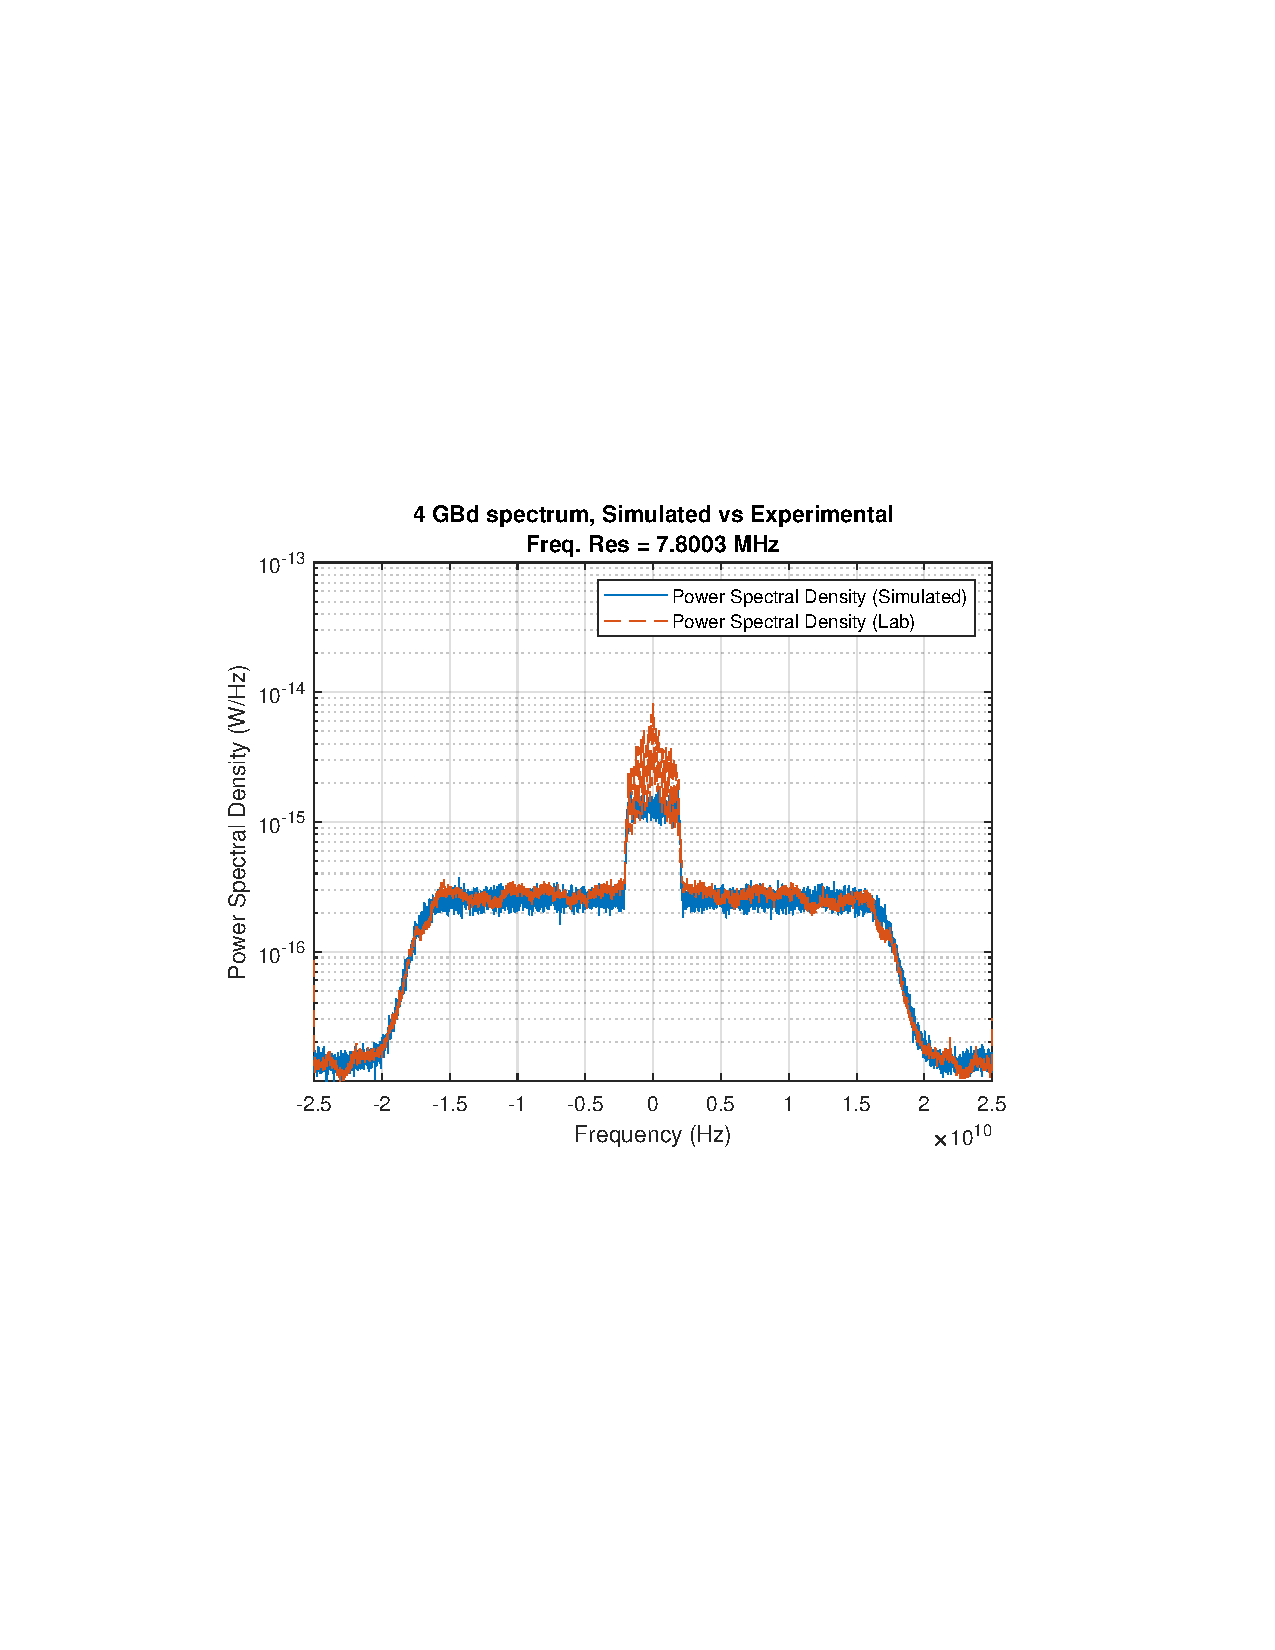
\includegraphics[clip, trim=2cm 8cm 2cm 8cm,
			width=1\textwidth]{./sdf/m_qam_system/figures/experimental/exampleComparisons/lbsmSpec4GBdEfOptNH_sameBer.pdf}
			\subcaption{\label{fig:specSuper4}}
		\end{minipage}
		\begin{minipage}{0.43\textwidth}
			\centering
			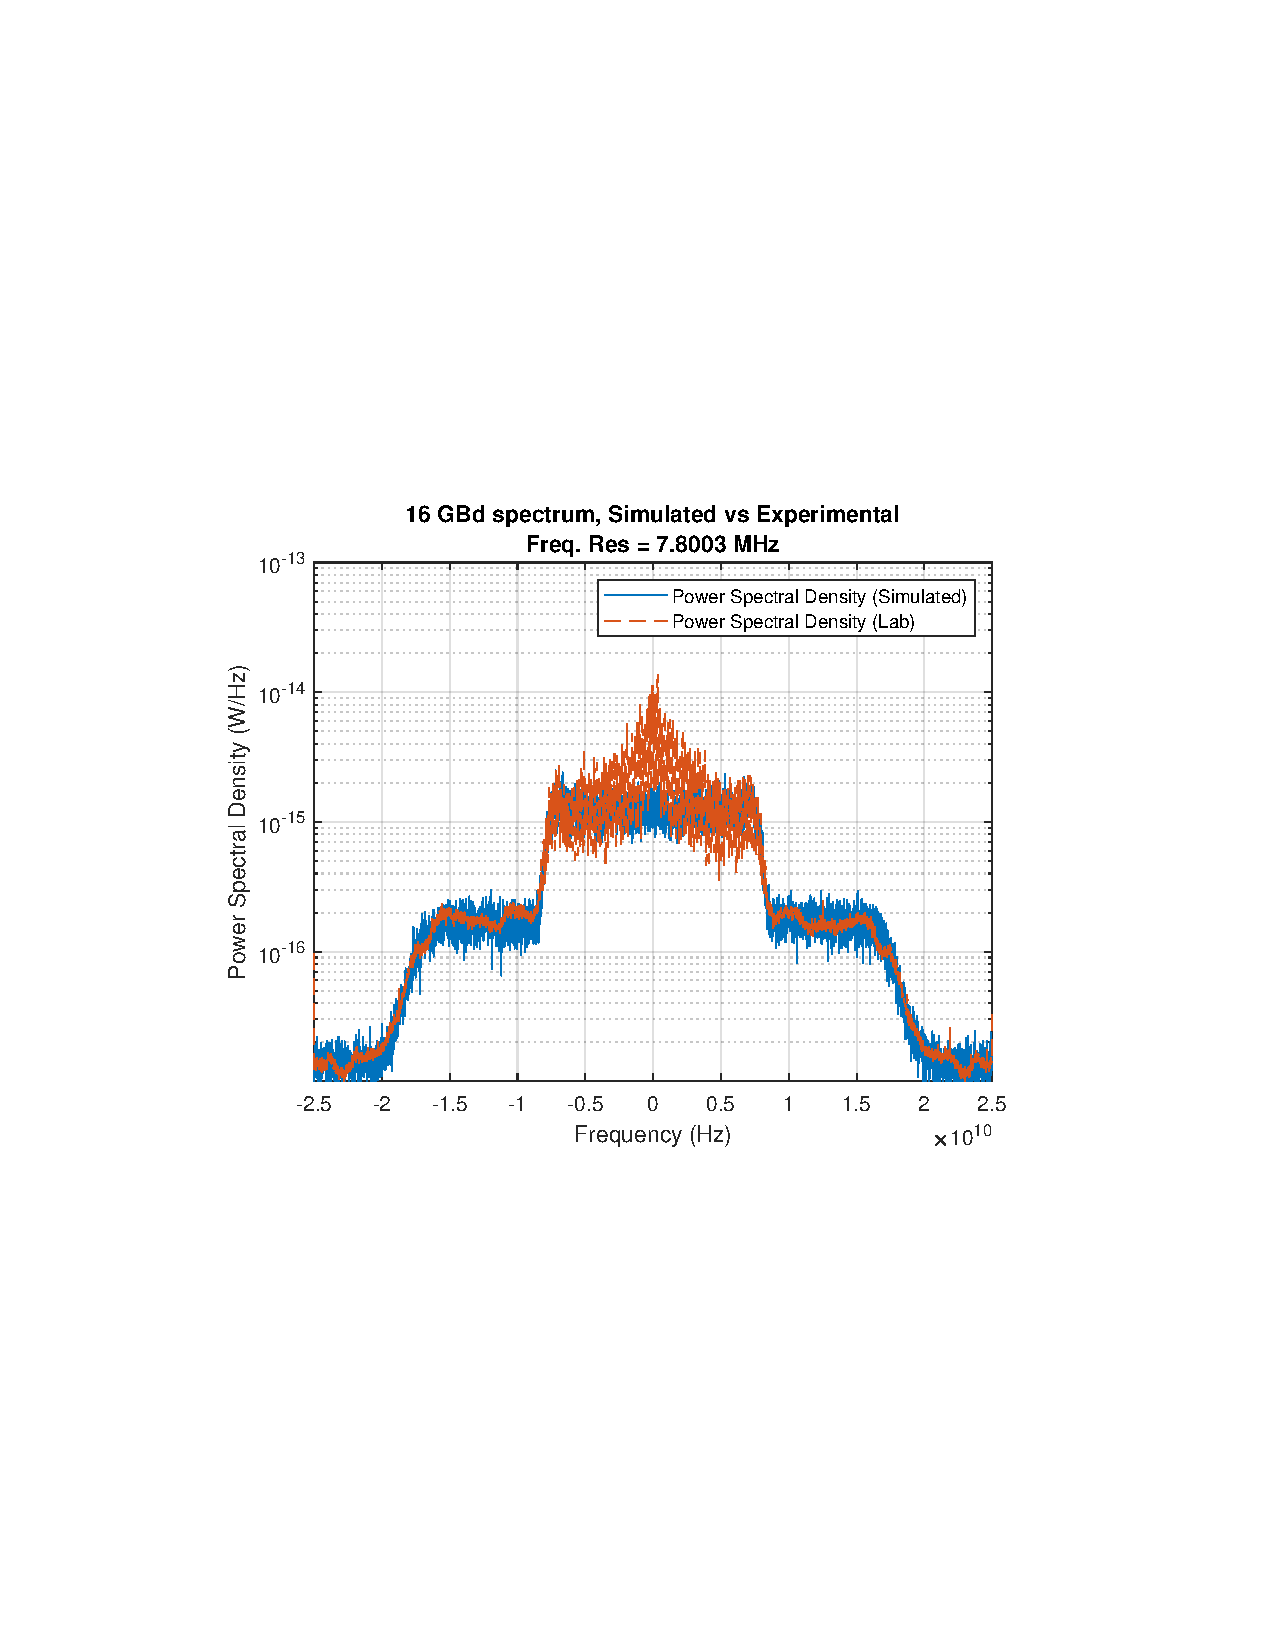
\includegraphics[clip, trim=2cm 8cm 2cm 8cm,
			width=1\textwidth]{./sdf/m_qam_system/figures/experimental/exampleComparisons/lbsmSpec16GBdEfOptNH.pdf}
			\subcaption{\label{fig:specSuper16}}
		\end{minipage}
		\caption{Comparison of spectra from simulated and experimental signals. 4 GBd signals on the
		left and 16 GBd on the right. The simulated and experimental signals produce the same BER.\label{fig:specSuperPosition}}
	\end{figure}


	Figure~\ref{fig:noises} shows the power spectrum of noise only signals,
	and their simulated counterparts, using the current simulation structure
	(optical white noise, electrical filter and electrical white noise after the
	electrical filter). The use filter is a contained least squares linear phase
	low pass filter, designed in MATLAB with the function \texttt{fircls1}. An IIR
	butterworth filter was previously tested but failed to keep the signal usable.
	It can be seen that some peaks are present in the lower frequencies. The
	same does not happen with the current simulation configuration. In addition to
	the peaks, the noise spectral density seems to increase as it approaches DC.

	\begin{figure}[H]
		\centering
		\begin{minipage}{0.43\textwidth}
			\centering
			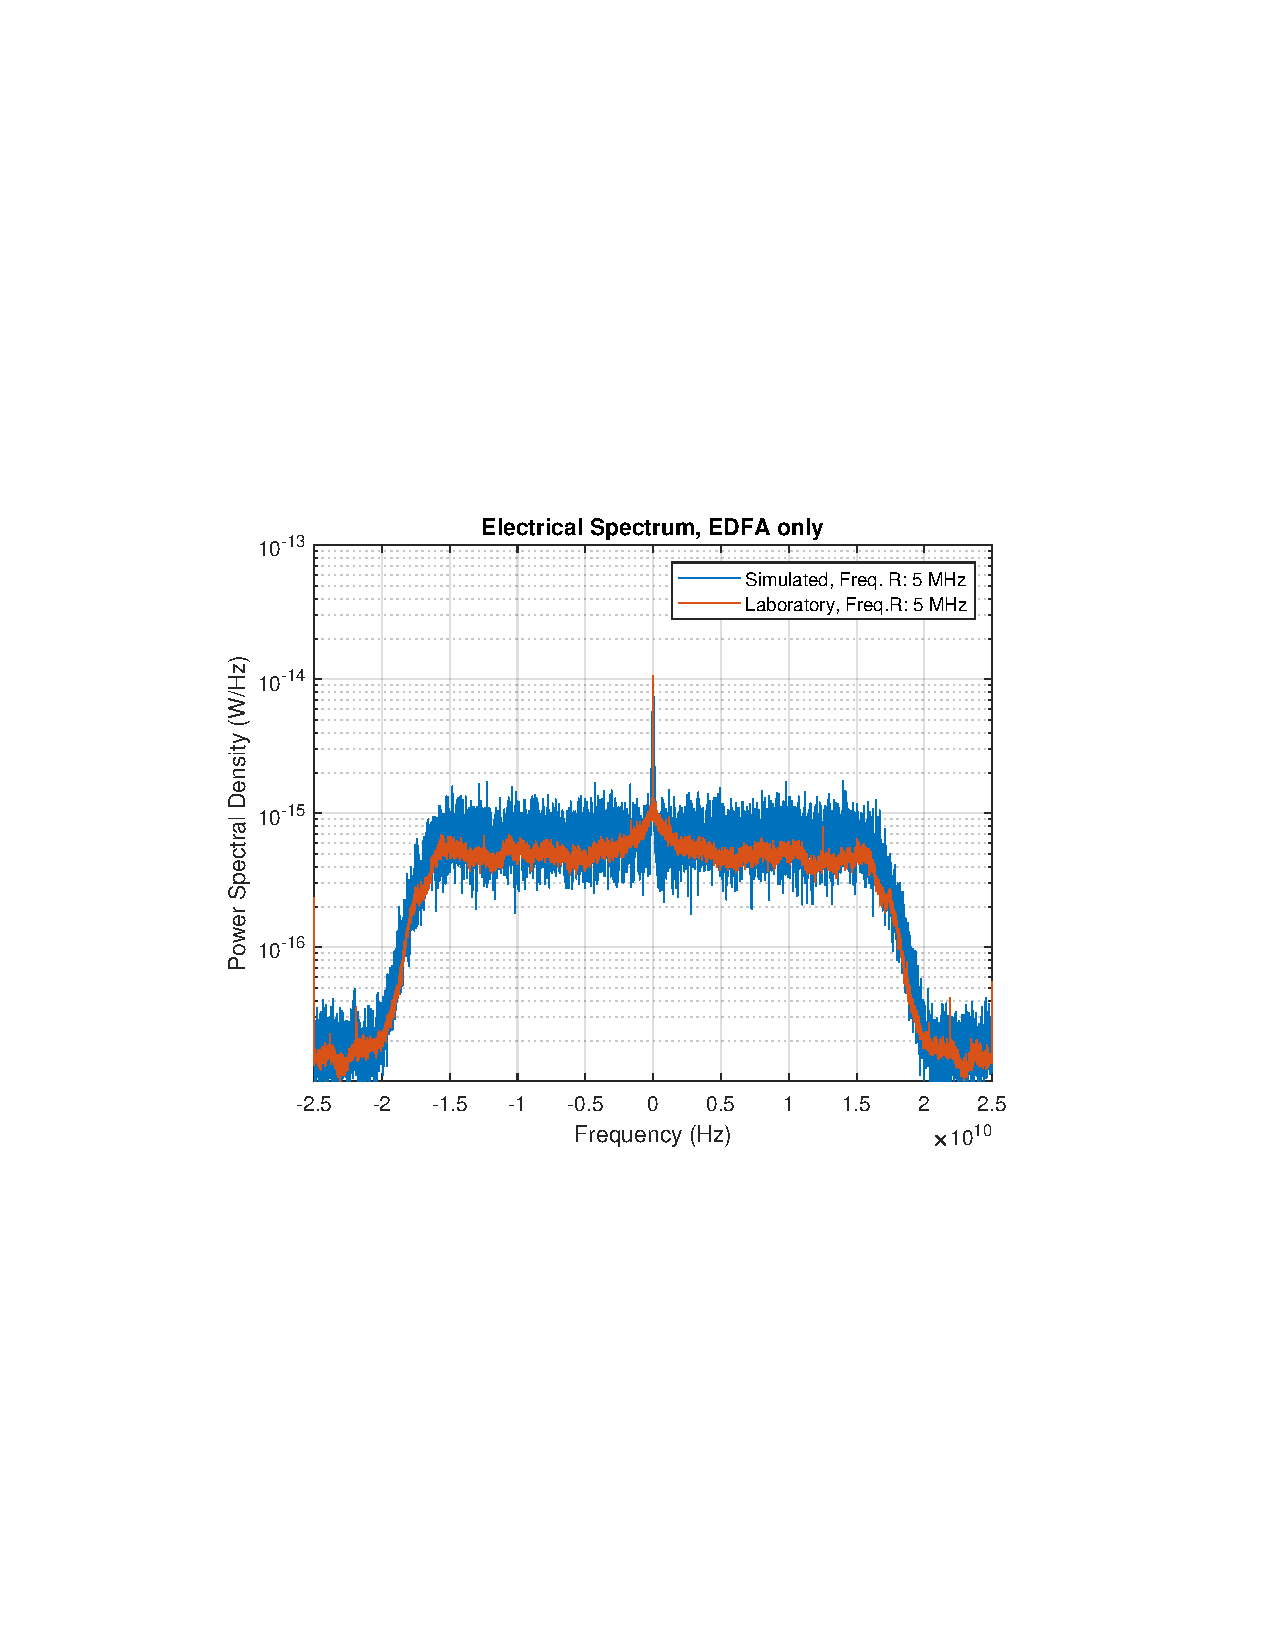
\includegraphics[clip, trim=3cm 8cm 3cm 8cm,
			width=1\textwidth]{./sdf/m_qam_system/figures/experimental/noiseSpectra/edfaOnly.pdf}
			\subcaption{\label{fig:oscNSimul}}
		\end{minipage}
		\begin{minipage}{0.43\textwidth}
			\centering
			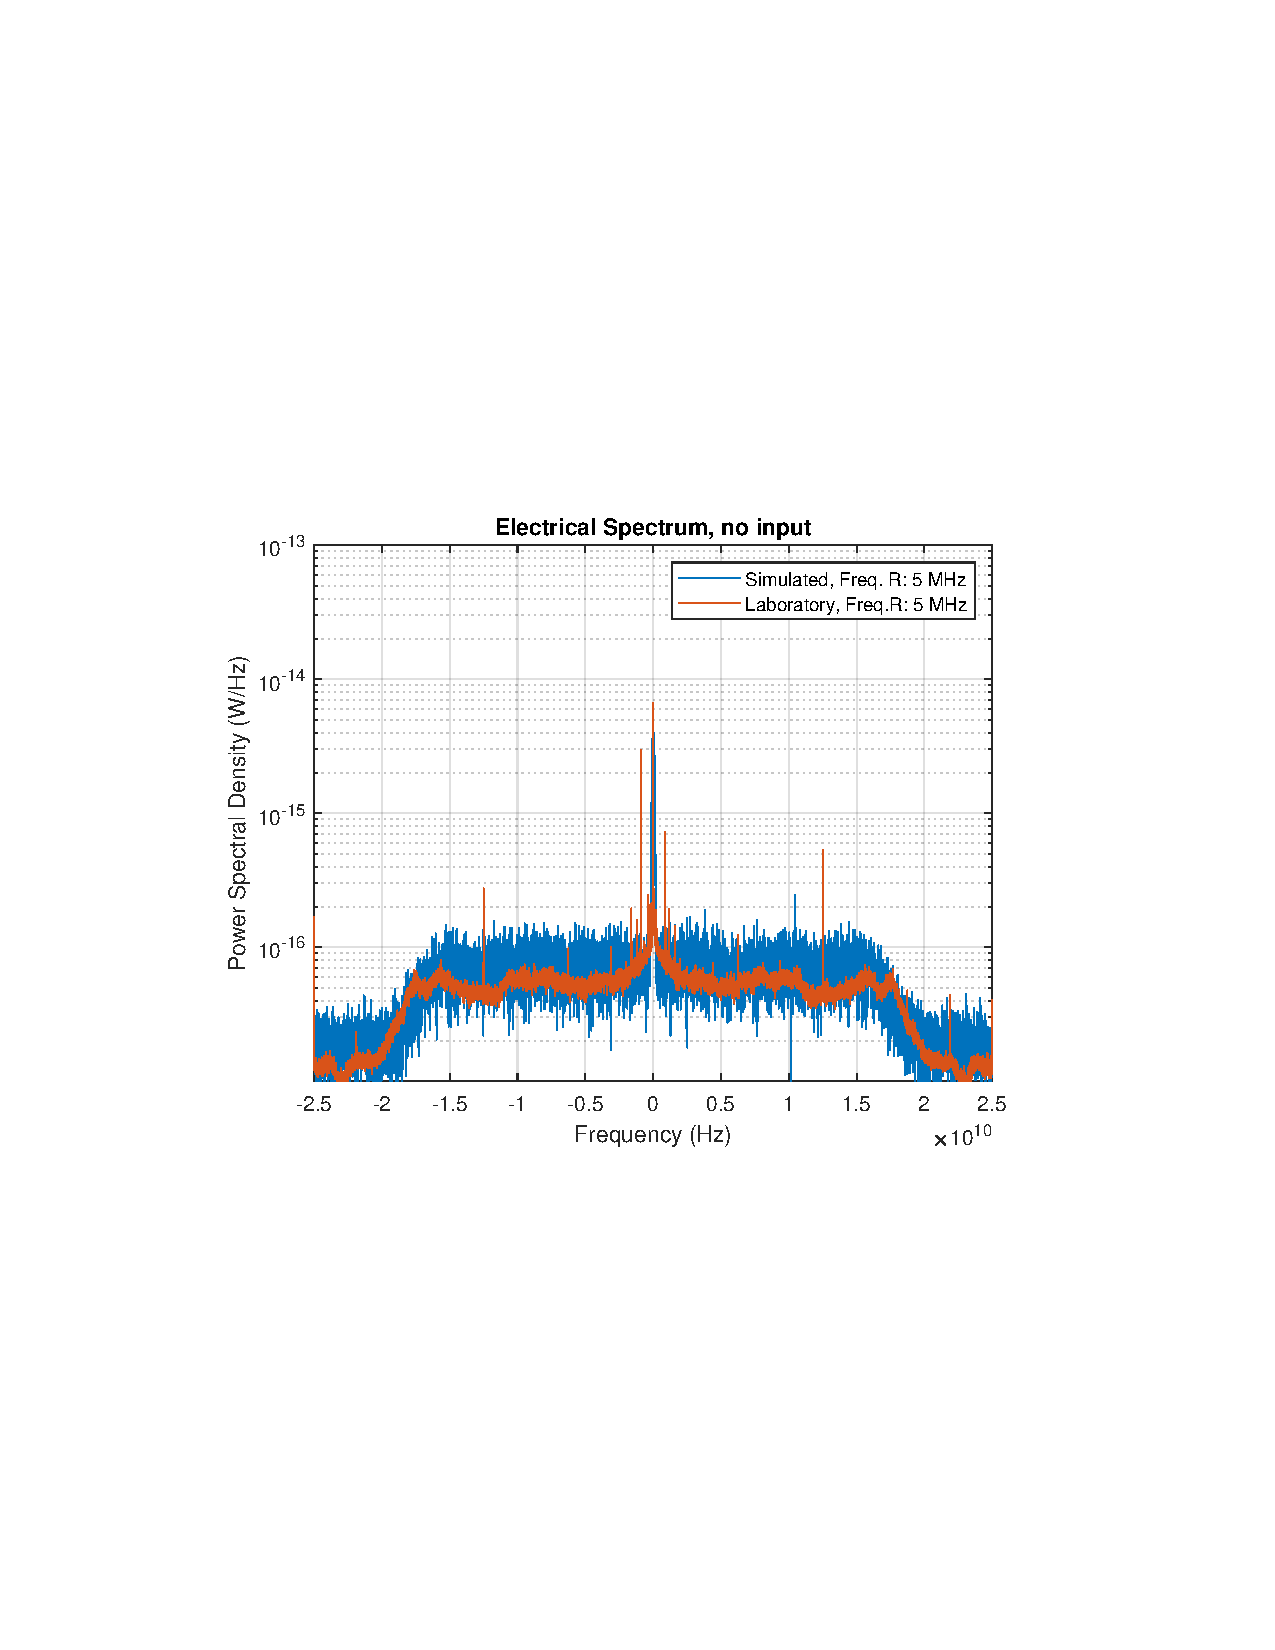
\includegraphics[clip, trim=3cm 8cm 3cm 8cm,
			width=1\textwidth]{./sdf/m_qam_system/figures/experimental/noiseSpectra/noInput.pdf}
			\subcaption{\label{fig:edfaNSimul}}
		\end{minipage}
		\caption{Power spectrum of the signal obtained when (a) the
			input signal is non-existing, and the local oscillator is turned off;
		(b) the input signal is made only of noise generated by the EDFA.\label{fig:noises}}
	\end{figure}

	In order to study the effects visible in the lower frequencies of the
	experimental spectra, several noise-only signals were acquired, with different
	sample rates. This allowed a better analysis of the situation, with greater
	emphasis on lower frequencies. There is a DC component always present, in the
	order of hundreds of microvolts. It can also immediately be seen that the
	measured noise power is independent of the sampling rate of the oscilloscope.
	Therefore, the noise spectral density is higher for lower sampling rates.

	At low enough sampling rates (below 6.25 MHz) no slope is noticed in the noise
	power spectral density ca be noticed. Its is possible that the vertical noise
	of the oscilloscope at ends up hiding the effect. At higher frequencies the
	effect is visible, but the noise spectral density does not keep continuously
	increasing in the lower frequencies. It actually only increases  up to the
	range of 10-100 KHz and the starts decreasing again. This does not appear to
	be a malfunction, but rather an intrinsic characteristic of the receiver.

	\begin{figure}[H]
		\centering
		\begin{minipage}{0.45\textwidth}
			\centering
			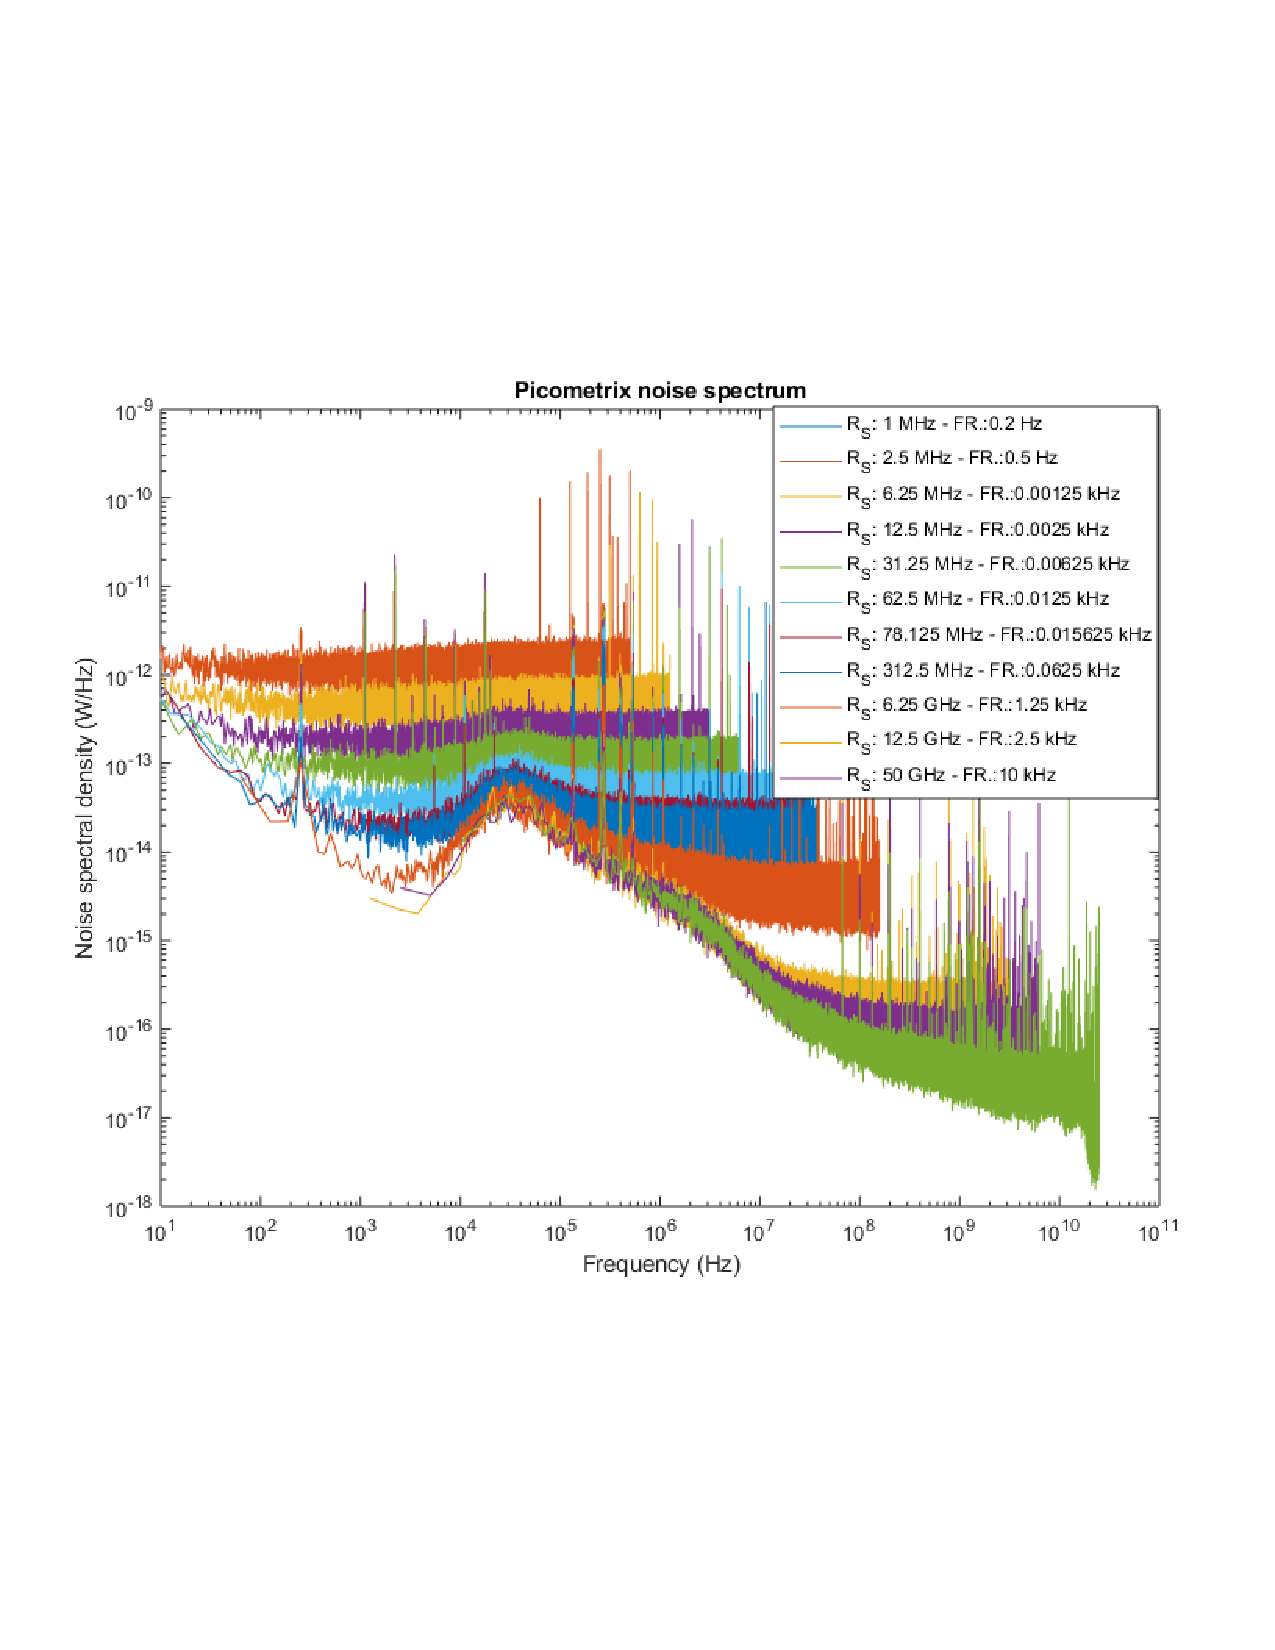
\includegraphics[clip, trim=1cm 6cm 1cm 6cm,
			width=0.9\textwidth]{./sdf/m_qam_system/figures/experimental/noiseSpectra/picoLogNoise2.pdf}
			\subcaption{\label{fig:noise5g}}
		\end{minipage}
		\begin{minipage}{0.45\textwidth}
			\centering
			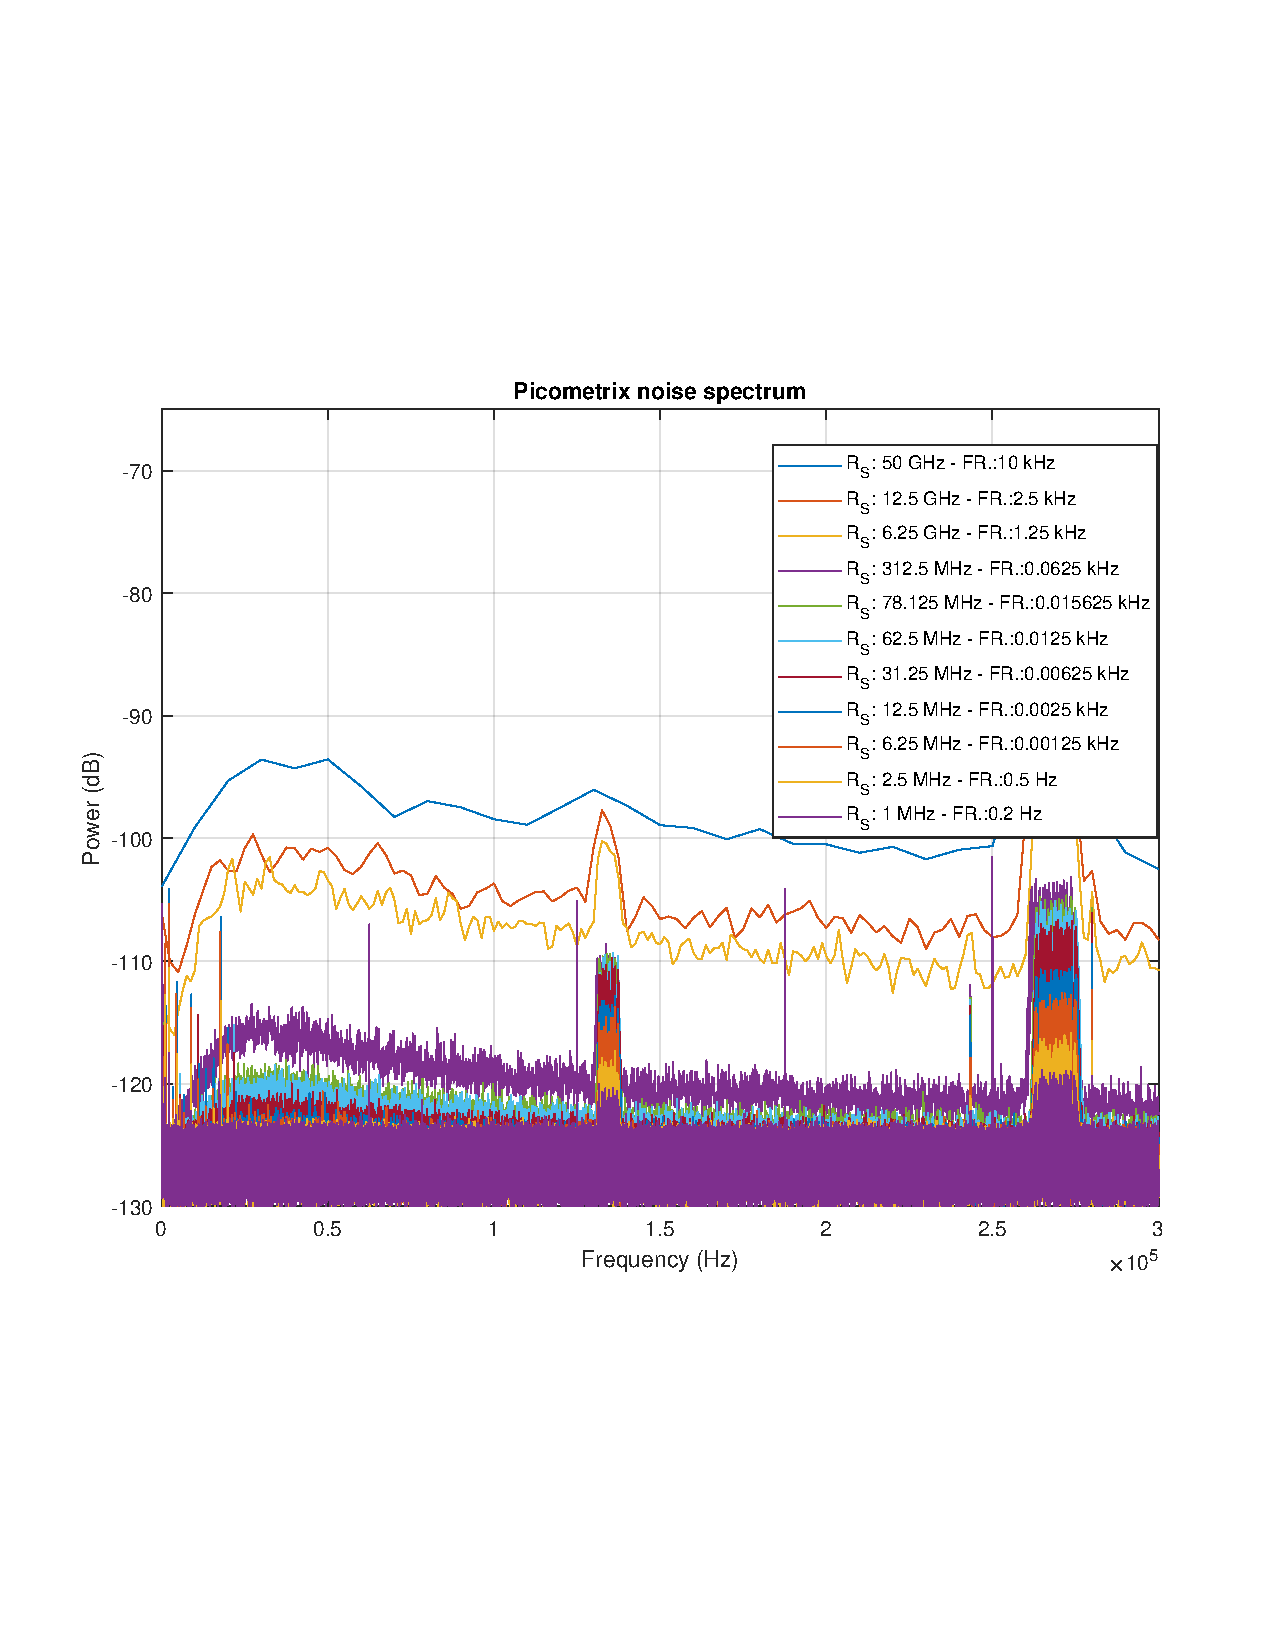
\includegraphics[clip, trim=1cm 6cm 1cm 6cm,
			width=0.9\textwidth]{./sdf/m_qam_system/figures/experimental/noiseSpectra/picoNoiseComp.pdf}
			\subcaption{\label{fig:noise50m}}
		\end{minipage}
		\caption{Noise spectra at various sample rates (a) Logarithmic plot, normalized to frequency resolution (b) Linear frequency scale, not normalized.\label{fig:noiseVariations}}
	\end{figure}

	Two more aspects should be considered in the transmission process. The signal
	appears to be different from the expected starting early on the transmission
	process. The electrical waveform generated by the AWG is slightly different
	from the waveform it uses as a source for signal generation, particularly for
	frequencies lower than 1 GHz. On the other hand, most of the fault seems to be
	at the modulator, as the optical spectrum after modulation is the first point
	where the spectrum is really distorted.

	\begin{figure}[H]
		\centering
		\begin{minipage}{0.45\textwidth}
			\centering
			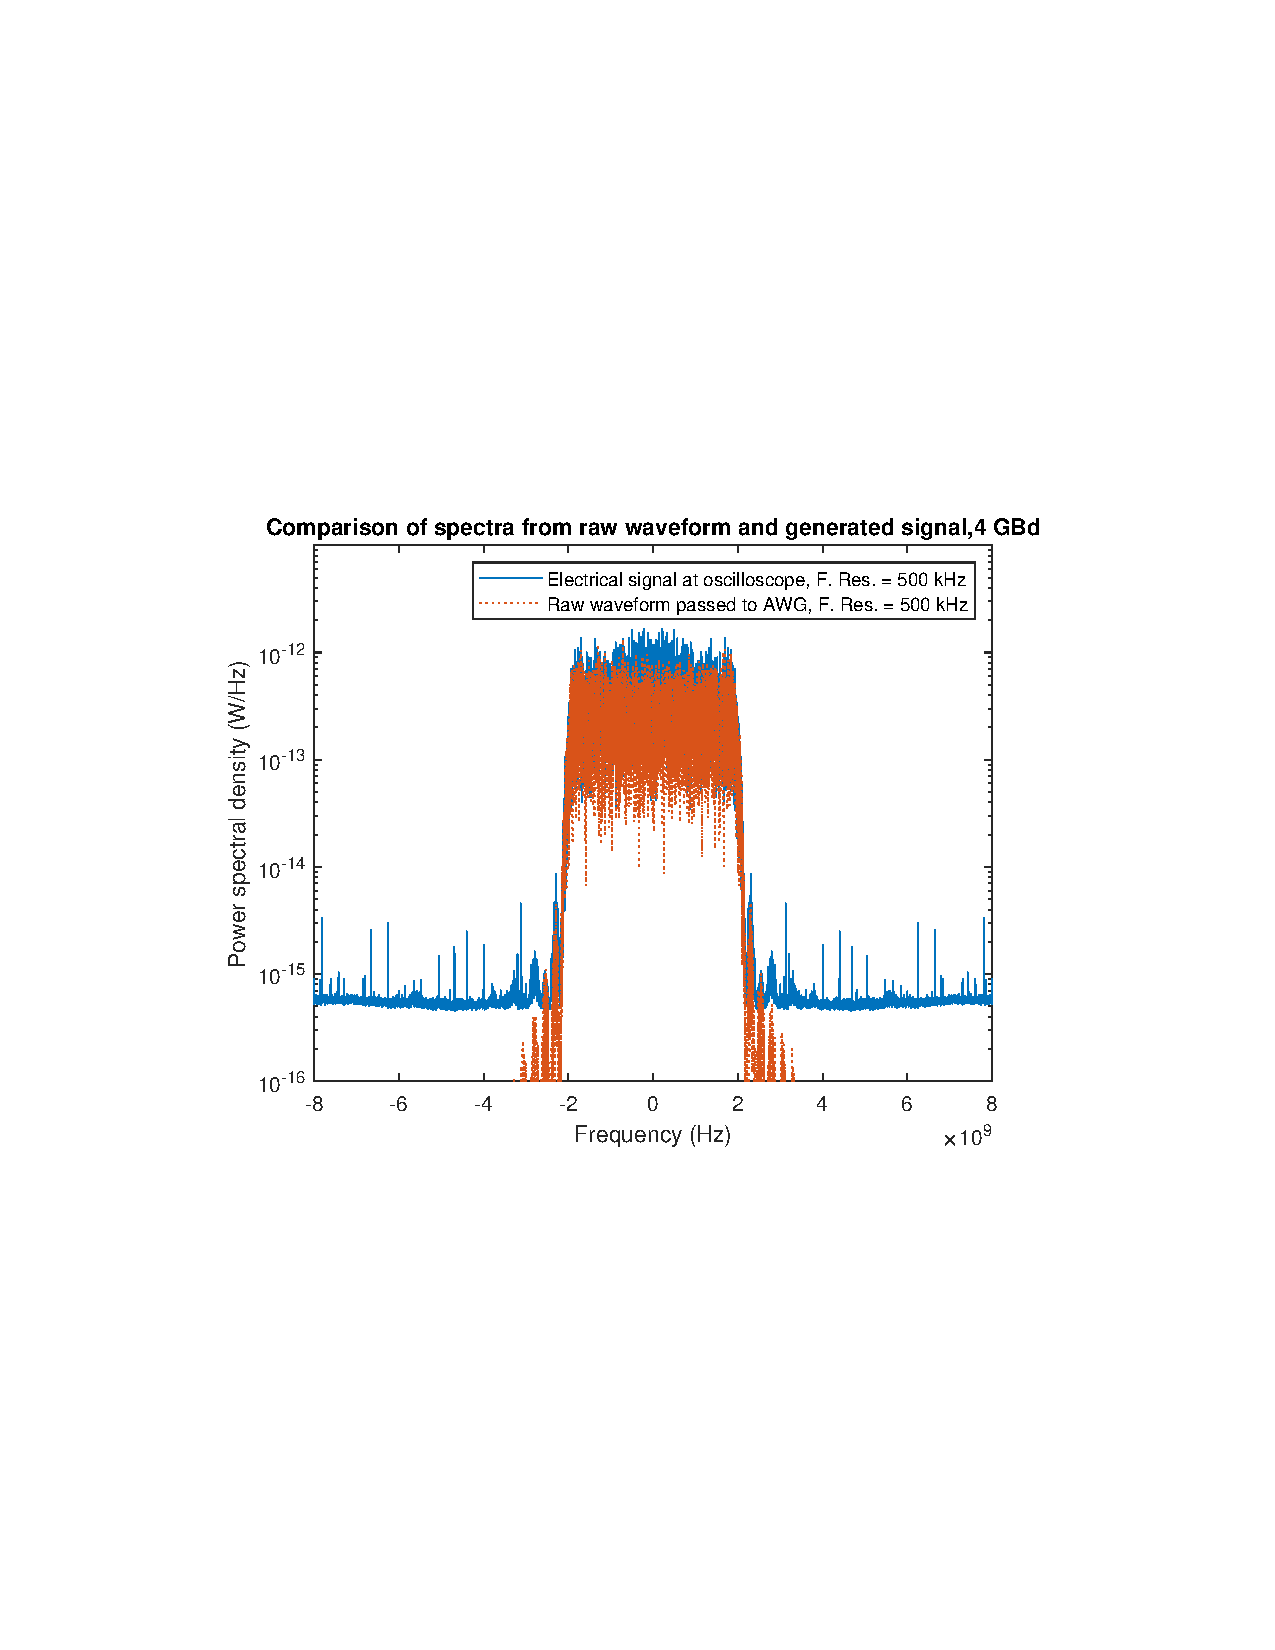
\includegraphics[clip, trim=4cm 8cm 4cm 8cm,
			width=0.9\textwidth]{./sdf/m_qam_system/figures/experimental/signalSpectra/awg4GBdComp.pdf}
			\subcaption{\label{fig:awg4gb}}
		\end{minipage}
		\begin{minipage}{0.45\textwidth}
			\centering
			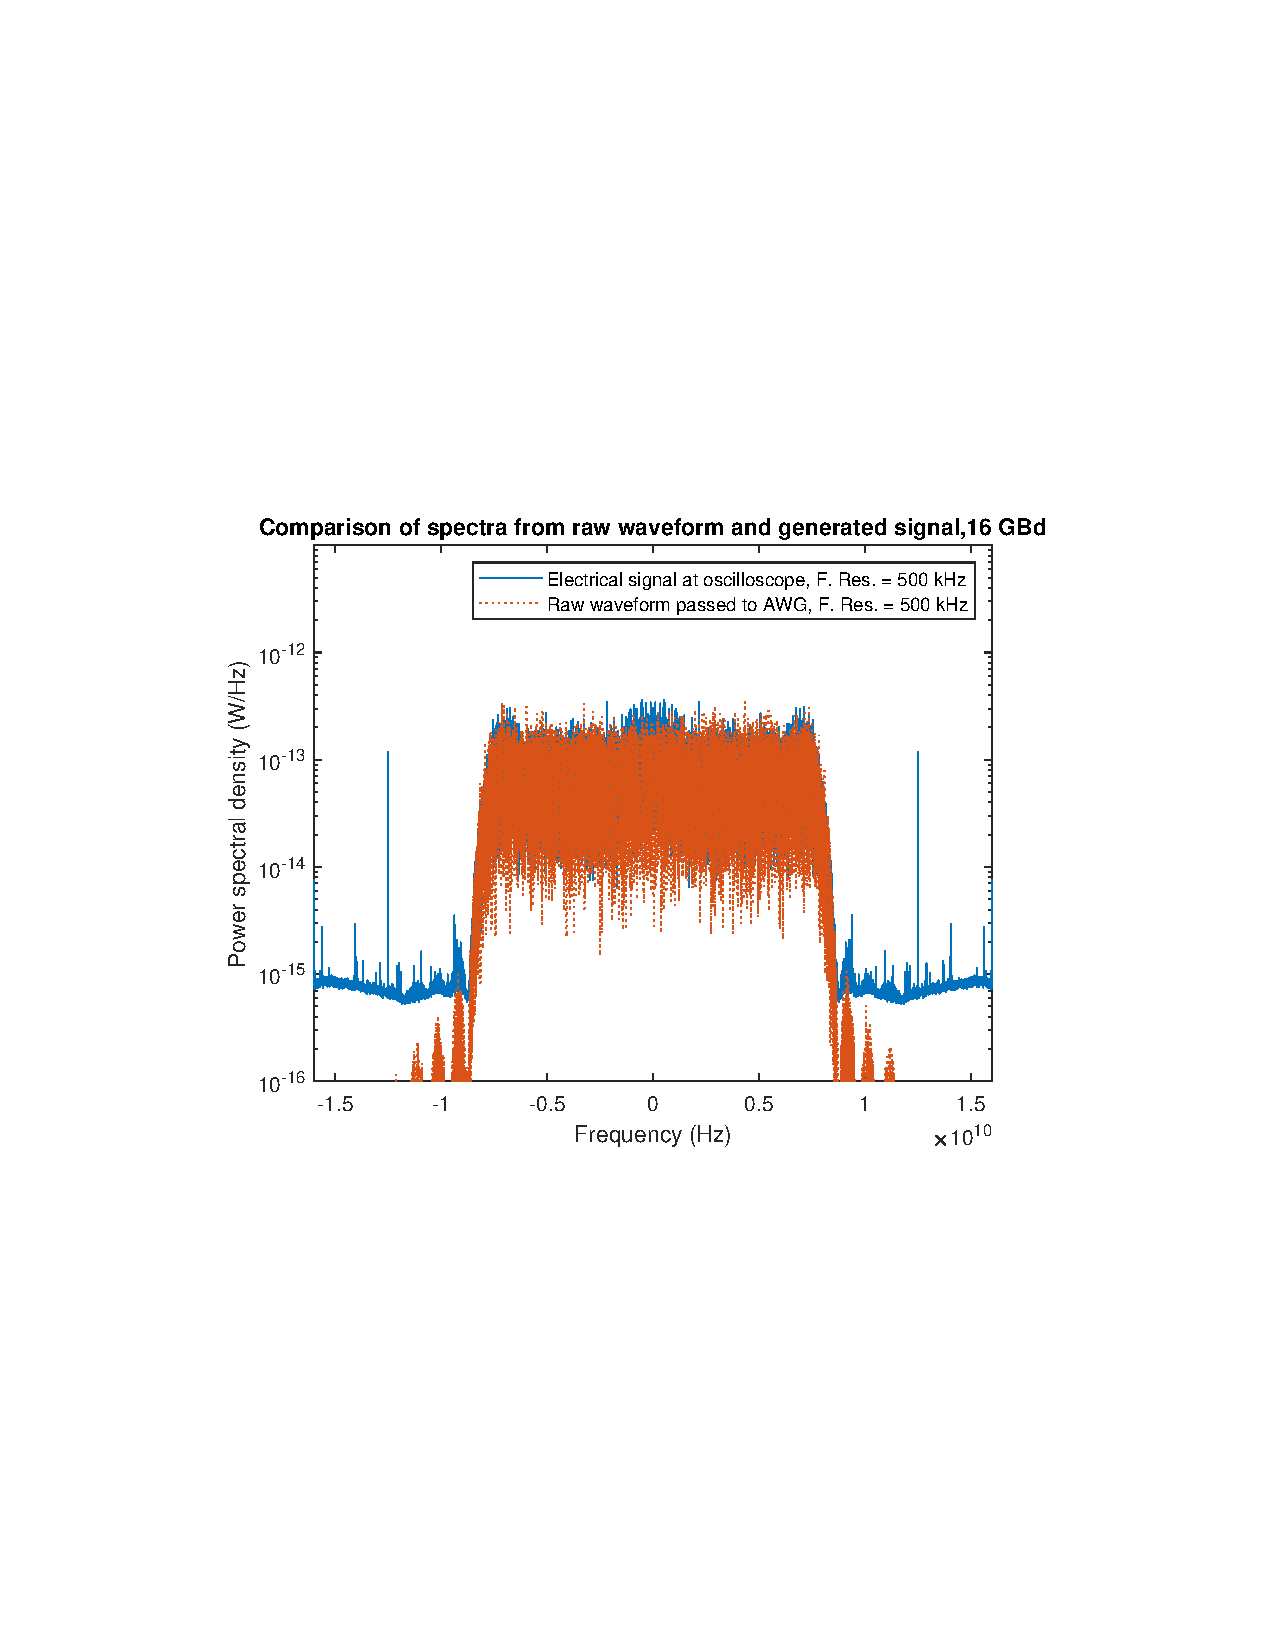
\includegraphics[clip, trim=4cm 8cm 4cm 8cm,
			width=0.9\textwidth]{./sdf/m_qam_system/figures/experimental/signalSpectra/awg16GBdComp.pdf}
			\subcaption{\label{fig:awg16gb}}
		\end{minipage}
		\caption{Spectra of electrical signals generated by the AWG compared to the original wabveforms\label{fig:awgvsraw}}
	\end{figure}

	\begin{figure}[H]
		\centering
		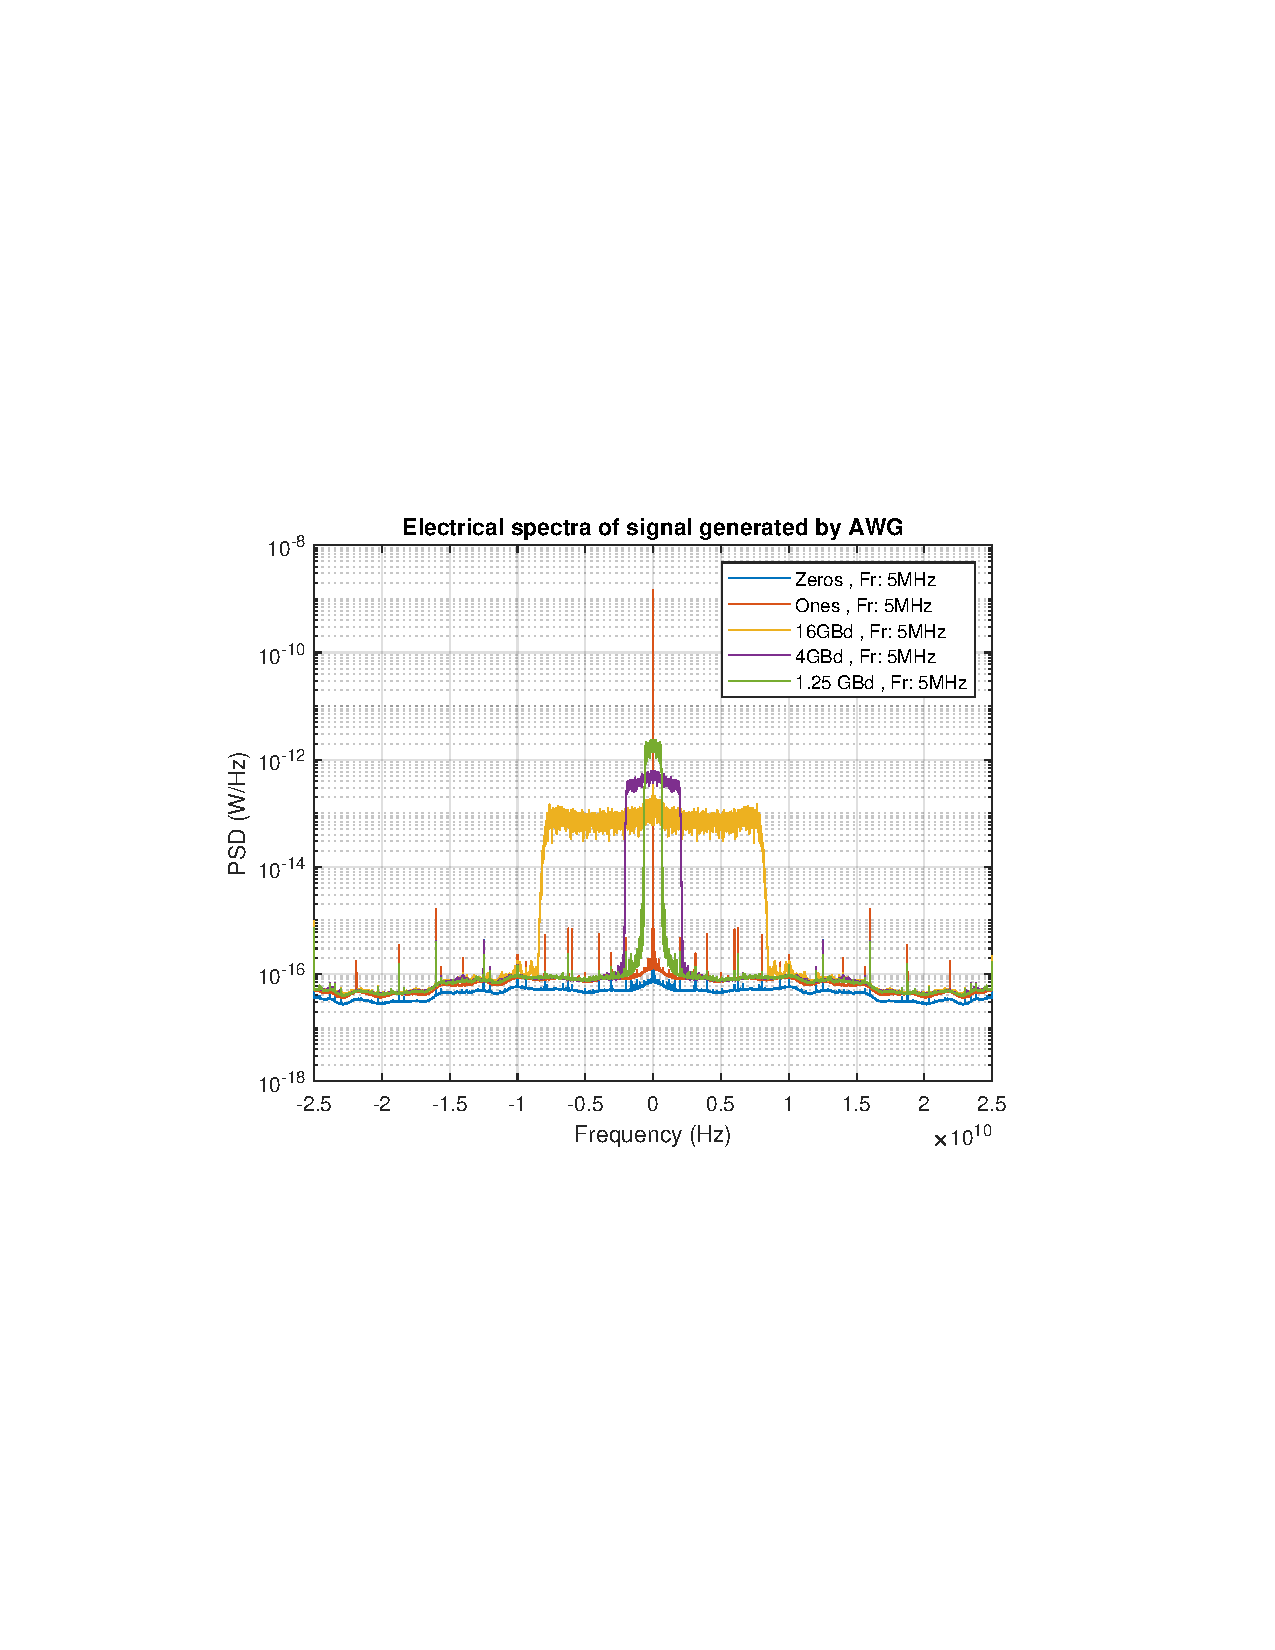
\includegraphics[clip, trim=3cm 8cm 3cm 8cm,
		width=0.7\textwidth]{./sdf/m_qam_system/figures/experimental/signalSpectra/AWG_spectra.pdf}
		\caption{Spectra of the electrical signals generated by the AWG.\label{fig:awgSpectra}}
	\end{figure}

	\begin{figure}[H]
		\centering
		\begin{minipage}{0.45\textwidth}
			\centering
			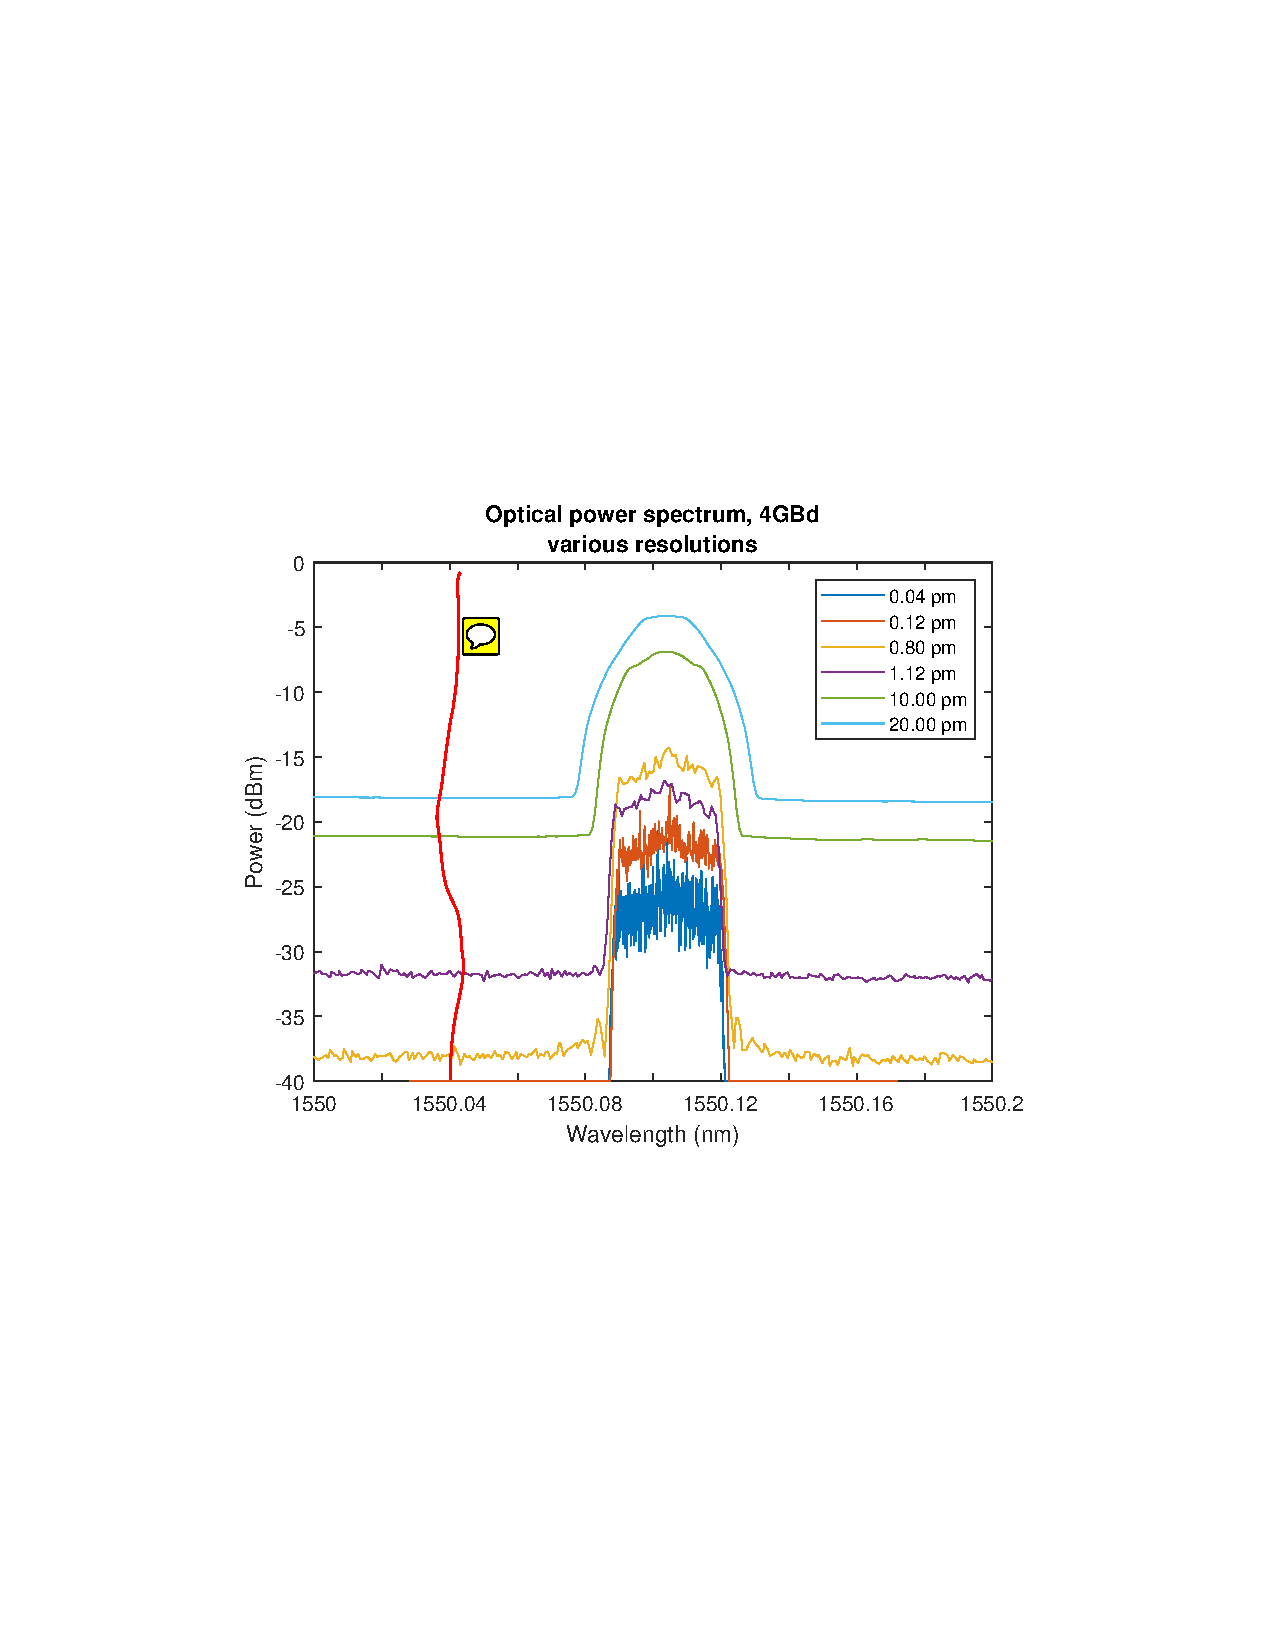
\includegraphics[clip, trim=4cm 8cm 4cm 8cm,
			width=0.9\textwidth]{./sdf/m_qam_system/figures/experimental/signalSpectra/4GBdSpectra.pdf}
			\subcaption{\label{fig:opt4gbres}}
		\end{minipage}
		\begin{minipage}{0.45\textwidth}
			\centering
			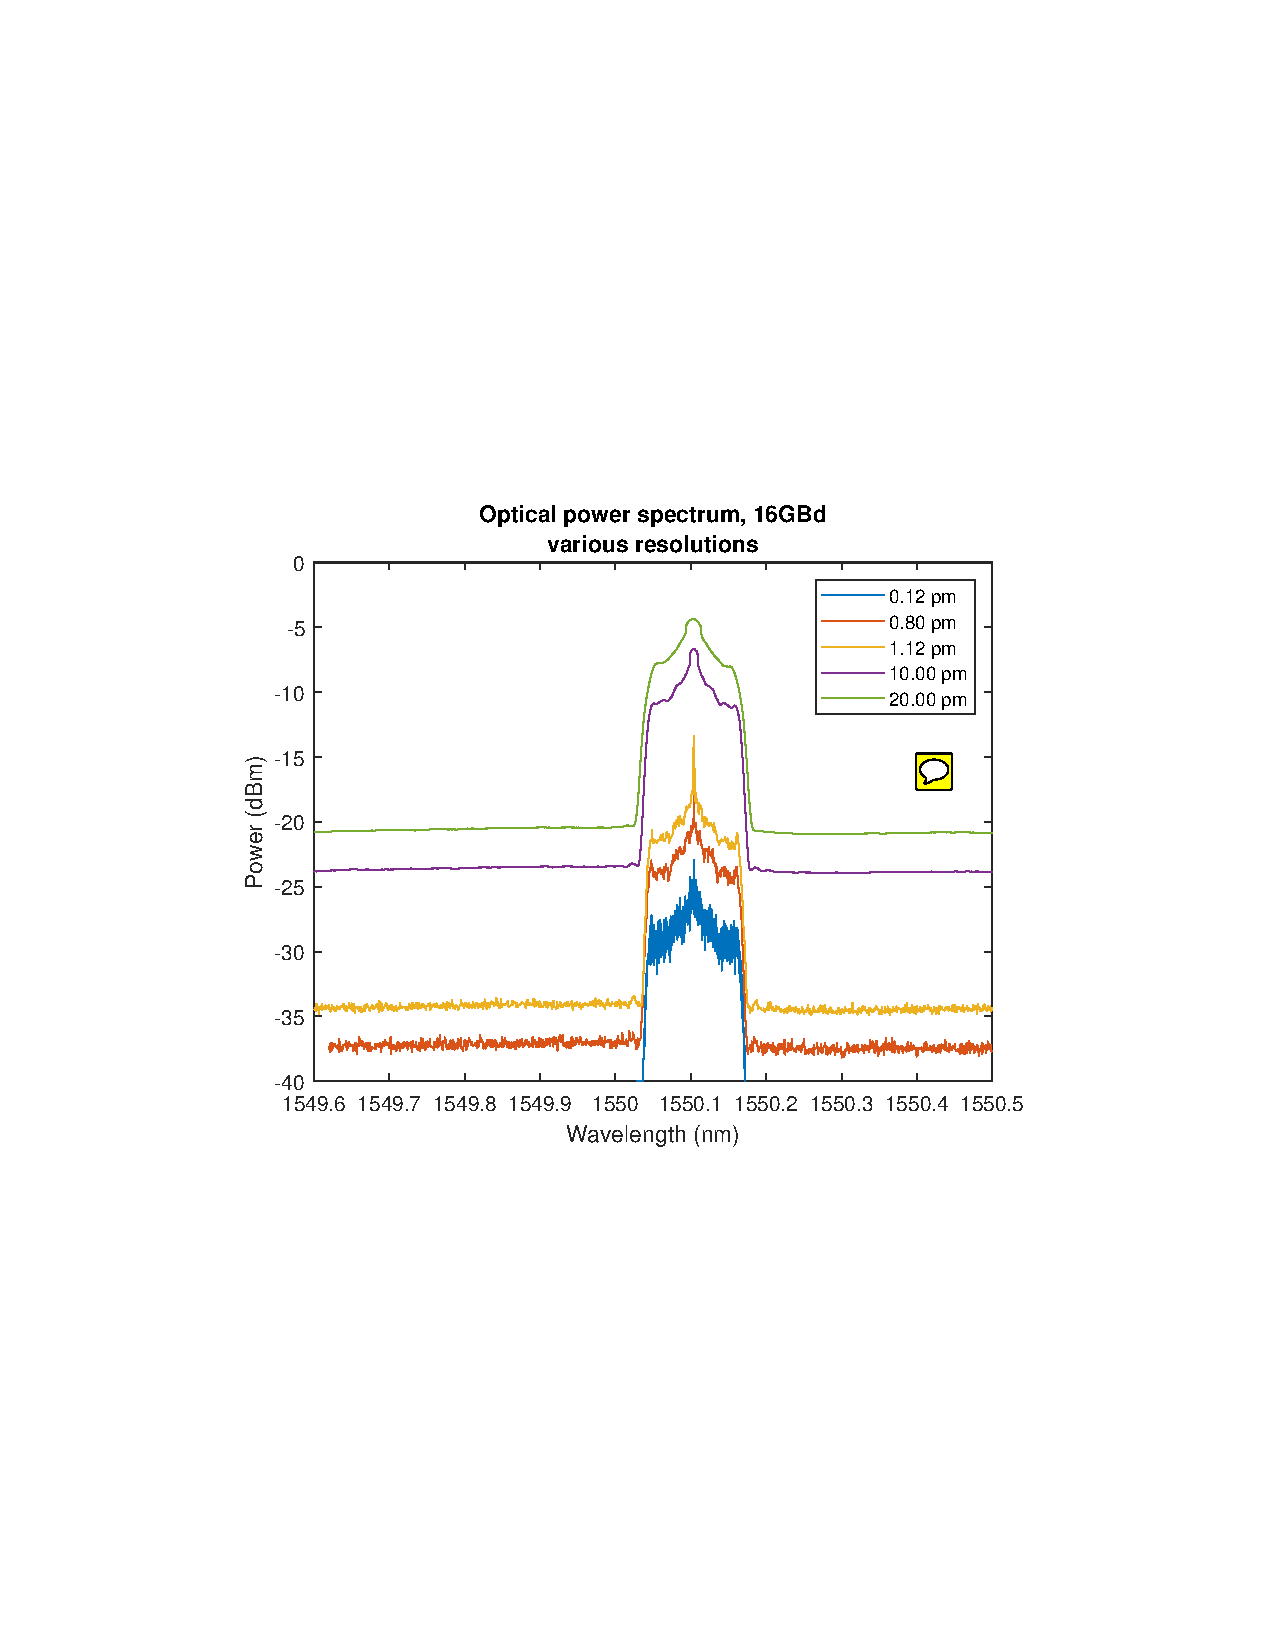
\includegraphics[clip, trim=4cm 8cm 4cm 8cm,
			width=0.9\textwidth]{./sdf/m_qam_system/figures/experimental/signalSpectra/16GBdSpectra.pdf}
			\subcaption{\label{fig:opt16gbres}}
		\end{minipage}
		\caption{Optical spectra of the modulated signals at different resolutions.\label{fig:optvarres}}
	\end{figure}


	These phenomena can help partially explain the deviation from the ideal curves
	that can be seen in the following sections.

	\subsubsection{Considerations about parameters and
	results}\label{sec:expValues}.
	Similarly to what was discussed in section~\ref{sec:simulValues}, we need to
	establish the origin of each value used to analyze the perfomance of the
	system. Using that section as a reference, we can say from the start that the
	estimated values and their origin are quite similar to the ones in the
	simulation. However, some differences are worth noting, due to differences
	between the simulation and the real world.
	In the following descriptions, keep in mind that the overall architecture of
	the setup is described in Figure~\ref{fig:experimental_mqam_setup}, and the
	specifications of each particular device are in the tables following the
	figure. With this in mind, the possible origins for the values to use are:


	\begin{itemize}
		\item Value defined in the equipment settings, such as transmitter power, or
			intrinsic to the used devices, such as bandwidth;
		\item Value obtained through direct measurement or calculations made using
			the optical signal at the Optical Spectrum Analyzer. This optical signal
			contains a conjunction of the modulated signal and noise generated by the
			EDFA, if available;
		\item Value measured or calculated offline using the waveform acquired
			with the oscilloscope connected to the coherent receiver; this is
			a digital representation of the electrical signal generated at the
			receiver, and is also the one used to apply the DSP and ultimately obtain
			the results. The sampling rate is 50 GHz, higher than any symbol rate.
	\end{itemize}

	Notice that there is a certain parallelism between the experimental
	measurements and the signals mentioned in section~\ref{sec:simulValues}. In
	particular, they were chosen in way that they can be studied as similarly as
	possible. For this reason, it is possible to measure the relevant parameters
	in a similar way. For instance, measuring the Q-Factor instead of the BER
	brings benefits similar to the ones described in that section. In
	addition, the $E_b/n_0$ or SNR values can be estimated in the same way as in
	the simulation, where it's easier to keep track of the source of each noise or
	imperfection source. Therefore, the $E_b/n_0$ and SNR values used are measured
	in the same points: at the OSA or using the waveform acquired at the
	oscilloscope, using the same processes described in
	section~\ref{sec:simulValues}. However, unlike in the simulation, it is hard
	to estimate the SNR of the electrical signal using Matzner's method, as
	nonlinearities would need to be compensated previously. Nevertheless, methods
	based on spectral analysis work well in the simulation or in the lab setup,
	and so they are used in both. Further information can be found in
	Section~\ref{sec:simulValues}.

	Overall, on the results presented here, only $E_b/n_0$ is used in the BER
	plots. This $E_b/n_0$ can be estimated on any of the two cases mentioned
	above, and the source will be identified in the caption or legend. If the EDFA
	is used to generate noise, the $E_b/n_0$ is measured in the OSA, and the value
	is referred to as "Optical $E_b/n_0$". Otherwise, if no EDFA is present,
	it cannot be measured in the optical domain, so it measured through the
	spectrum of the electrical signal, as described in
	section~\ref{sec:simulValues}, and referred to as "Electrical $E_b/n_0$".
	This way, it is possible to accurately study both cases.

	It is worth noting that, when using the "Optical $E_b/n_0$", it does not
	encompass all noise sources in the signal. This value only considers the optical noise
	generated by the EDFA, ignoring all electrical noise sources. Also, it is
	important to remember that this analysis considers that all nonlinearities in
	the signal can be neglected or compensated by DSP (a reasonable assumption
	used in~\cite{crognale14}). It is also assumed that the receiver is perfectly
	balanced. While this is a bit more unrealistic, it is the case used in the simulation.

	\subsection{Homodyne Detection}
	Using the same laser source for transmitting the signal and acting as local
	oscillator, the frequencies of the carrier and local oscillator are always
	synchronized. Therefore, using this configuration there should be no need for
	frequency estimation or phase corrections. However, some DSP is still
	required.

	The final constellations were obtained resorting to the OptDSP libraries for
	signal processing. The post-processing is done offline and in several stages.
	It starts by removing the existing skew between the in-phase and quadrature
	components.These components are acquired in different channels of the
	oscilloscope with a given timing skew that requires correction. The DC
	component of the signal is also removed. Afterwards, Gram-Schmidt
	Orthogonalization is done to compensate possible quadrature imbalances A
	matched filter is then used to improve the signal's SNR, as discussed
	previously. A constant modulus algorithm MIMO 2x2 adaptive equalizer is used
	to compensate for the channel distortion of the transmitted signal. Due to the
	homodyne configuration, there was no need to perform frequency or phase
	corrections. Lastly, a Least-Mean-Square MIMO 4x4 is used for further adaptive
	equalization.

	Figure~\ref{fig:ebBerH} shows the BER curves obtained for 16, 4 and 1.25~GBd signals.The
	theoretical curves were obtained resorting to equation~\ref{eq:berMod}.

	\begin{figure}[H]
		\centering
		\begin{minipage}{0.49\textwidth}
			\centering
			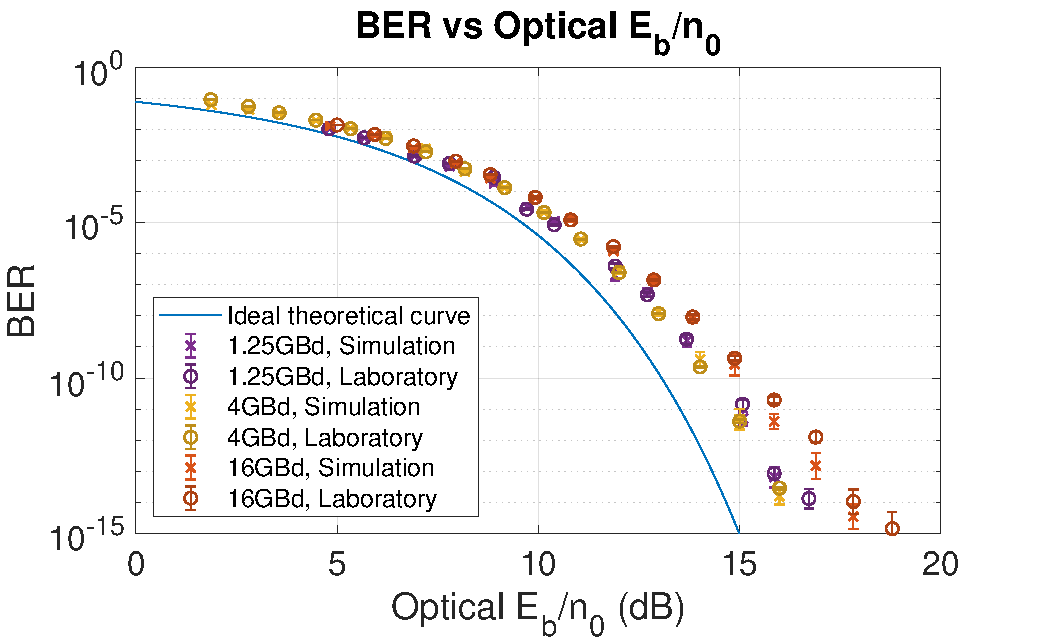
\includegraphics[width=\textwidth]{./sdf/m_qam_system/figures/experimental/results/general/test2.pdf}
%			\includegraphics[width=1\textwidth]
%			{./sdf/m_qam_system/figures/berPlots/1217/OpticalEbn0VsBER.pdf}
			\subcaption{\label{fig:optEbBer}}
		\end{minipage}
		\begin{minipage}{0.49\textwidth}
			\centering
			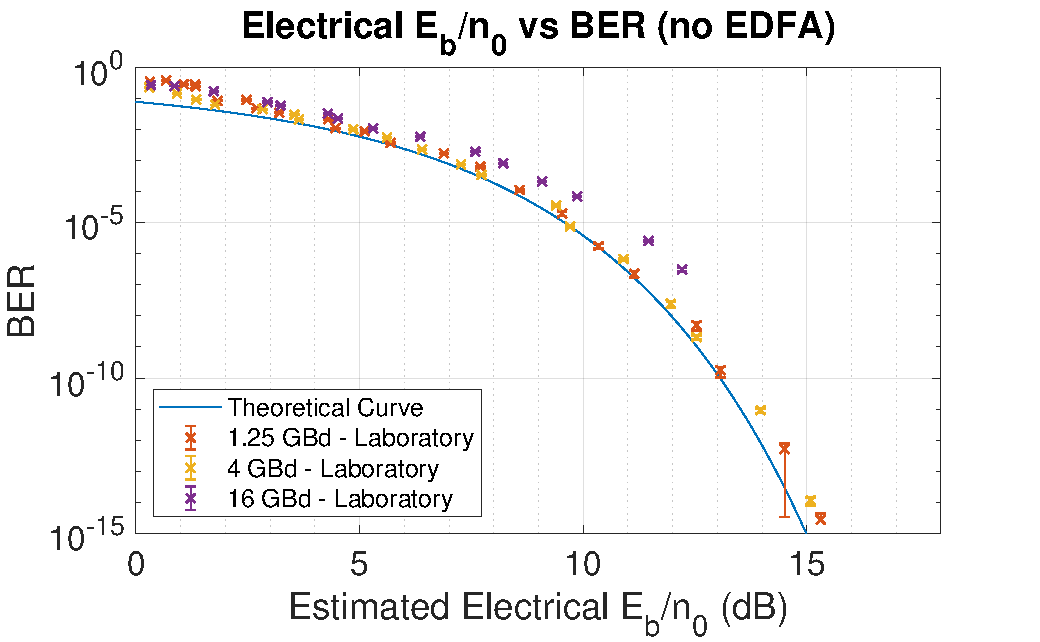
\includegraphics[width=\textwidth]{./sdf/m_qam_system/figures/experimental/results/general/test1.pdf}
			\subcaption{\label{fig:elEbBer}}
		\end{minipage}
		\caption{Comparison of theoretical BER curves against obtained results.
			Optical $E_b/n_0$ calculated through the optical spectrum, electrical
			$E_b/n_0$ estimated from the raw waveforms obtained at the oscilloscope,
			through spectral analysis of the acquired signal. Locally generated local
			oscillator .\label{fig:ebBerH}}
	\end{figure}

	The $E_b/n_0$ used to plot the experimental data points in
	Figure~\ref{fig:ebBerH} is estimated offline. Some further comments on the
	results follow in the sections of the respective symbol rate.


	\subsubsection{16 GBd Signal}

	Figures~\ref{fig:16GBdinitHm} to~\ref{fig:16GBdFinalHm} show the eye diagrams and the spectrum of the signals at every stage of the DSP process. The process is similar to the described for the intradyne configuration, but without phase or frequency corrections.

	\begin{figure}[H]
		\centering
		\begin{minipage}{0.3\textwidth}
			\centering
			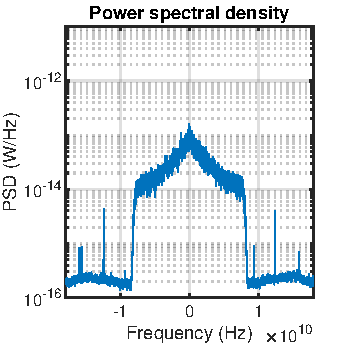
\includegraphics[width=1\textwidth]
			{./sdf/m_qam_system/figures/experimental/results/DSP_homodyne/0noEDFA_16_homodyne_16_6_spectrum.pdf}\\
			\label{fig:16GBdEyeBefFecHm}
		\end{minipage}
		\begin{minipage}{0.3\textwidth}
			\centering
			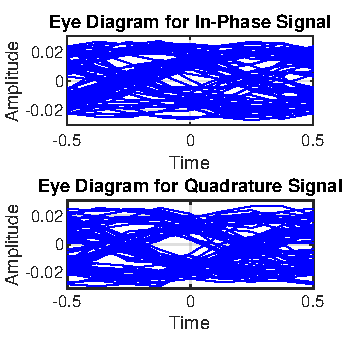
\includegraphics[width=1\textwidth]
			{./sdf/m_qam_system/figures/experimental/results/DSP_homodyne/0noEDFA_16_homodyne_16_6_eye.pdf}
			\label{fig:16GBdSpecBefFecHm}
		\end{minipage}
		\begin{minipage}{0.3\textwidth}
			\centering
			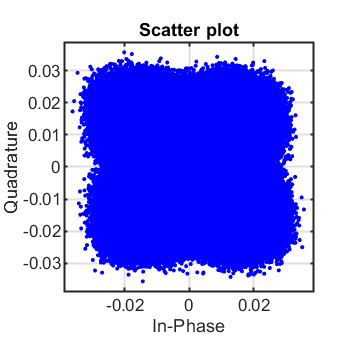
\includegraphics[width=1\textwidth]
			{./sdf/m_qam_system/figures/experimental/results/DSP_homodyne/0noEDFA_16_homodyne_16_6_const.pdf}\\
			\label{fig:16GBdSpecBefFecCHm}
		\end{minipage}
		\caption{Initial spectrum, eye Diagram, and constellation of the original
			signal obtained at the oscilloscope. Input signal power immediately before the
		coherent receiver was -16.6 dBm.}
		\label{fig:16GBdinitHm}
	\end{figure}


	\begin{figure}[H]
		\centering
		\begin{minipage}{0.30\textwidth}
			\centering
			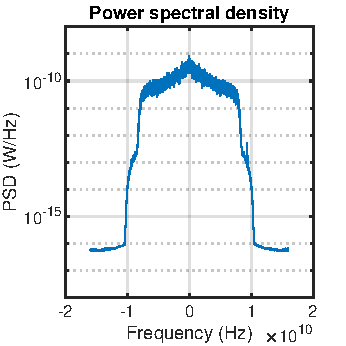
\includegraphics[ width=1\textwidth]
			{./sdf/m_qam_system/figures/experimental/results/DSP_homodyne/2noEDFA_16_homodyne_16_6_spectrum.pdf}\\
			\label{fig:16GBdEyeMf}
		\end{minipage}
		\begin{minipage}{0.30\textwidth}
			\centering
			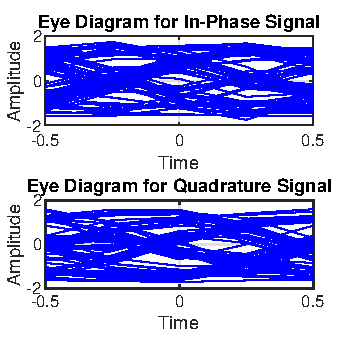
\includegraphics[ width=1\textwidth]
			{./sdf/m_qam_system/figures/experimental/results/DSP_homodyne/2noEDFA_16_homodyne_16_6_eye.pdf}
			\label{fig:16GBdSpecMF}
		\end{minipage}
		\begin{minipage}{0.30\textwidth}
			\centering
			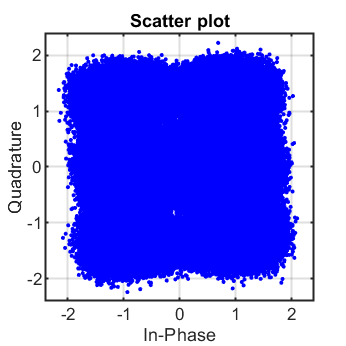
\includegraphics[width=1\textwidth]
			{./sdf/m_qam_system/figures/experimental/results/DSP_homodyne/2noEDFA_16_homodyne_16_6_const.pdf}\\
			\label{fig:16GBdSpecBefFec}
		\end{minipage}
		\caption{Spectrum, eye-diagram and constellation after applying front-end corrections, matched filtering and resampling to $2 S_R$.}
		\label{fig:16GBMFHm}
	\end{figure}


	\begin{figure}[H]
		\centering
		\begin{minipage}{0.30\textwidth}
			\centering
			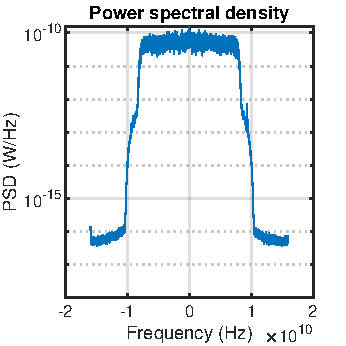
\includegraphics[ width=1\textwidth]
			{./sdf/m_qam_system/figures/experimental/results/DSP_homodyne/3noEDFA_16_homodyne_16_6_spectrum.pdf}\\
			\label{fig:16GBdEyeMf}
		\end{minipage}
		\begin{minipage}{0.30\textwidth}
			\centering
			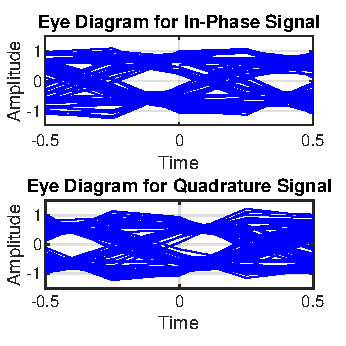
\includegraphics[ width=1\textwidth]
			{./sdf/m_qam_system/figures/experimental/results/DSP_homodyne/3noEDFA_16_homodyne_16_6_eye.pdf}
			\label{fig:16GBdSpecMF}
		\end{minipage}
		\begin{minipage}{0.30\textwidth}
			\centering
			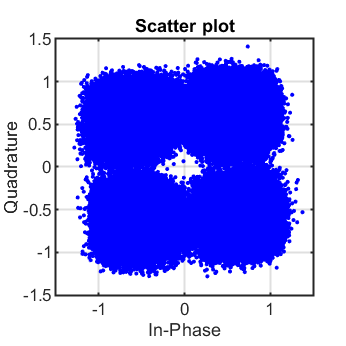
\includegraphics[width=1\textwidth]
			{./sdf/m_qam_system/figures/experimental/results/DSP_homodyne/3noEDFA_16_homodyne_16_6_const.pdf}\\
			\label{fig:16GBdSpecBefFec}
		\end{minipage}
		\caption{Spectrum, eye diagram and constellation after using a contant modulus
		algorithm.}
		\label{fig:16GBMFHm}
	\end{figure}


	\begin{figure}[H]
		\centering
		\begin{minipage}{0.30\textwidth}
			\centering
			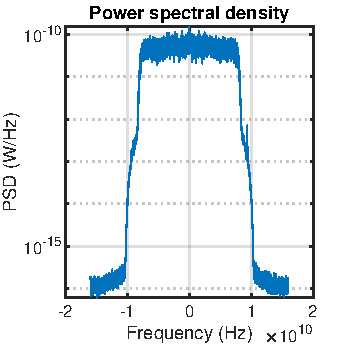
\includegraphics[ width=1\textwidth]
			{./sdf/m_qam_system/figures/experimental/results/DSP_homodyne/4noEDFA_16_homodyne_16_6_spectrum.pdf}\\
			\label{fig:16GBdEyeMf}
		\end{minipage}
		\begin{minipage}{0.30\textwidth}
			\centering
			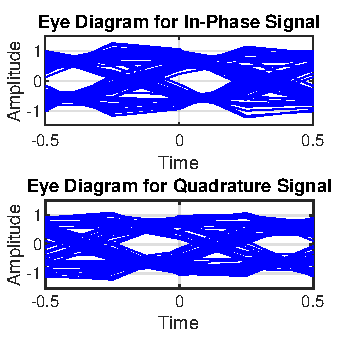
\includegraphics[ width=1\textwidth]
			{./sdf/m_qam_system/figures/experimental/results/DSP_homodyne/4noEDFA_16_homodyne_16_6_eye.pdf}
			\label{fig:16GBdSpecMF}
		\end{minipage}
		\begin{minipage}{0.30\textwidth}
			\centering
			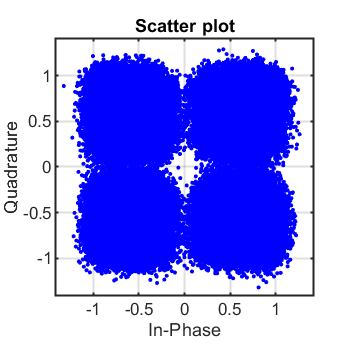
\includegraphics[width=1\textwidth]
			{./sdf/m_qam_system/figures/experimental/results/DSP_homodyne/4noEDFA_16_homodyne_16_6_const.pdf}\\
			\label{fig:16GBdSpecBefFec}
		\end{minipage}
		\caption{Spectrum, eye diagram and constellation after carrier-phase
		compensation.}
		\label{fig:16GBMFHm}
	\end{figure}


	\begin{figure}[H]
		\centering
		\begin{minipage}{0.30\textwidth}
			\centering
			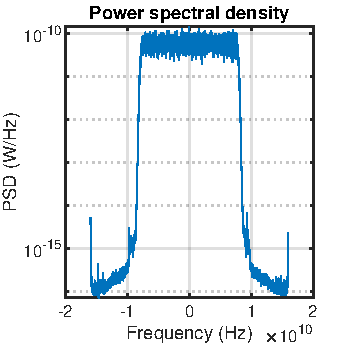
\includegraphics[ width=1\textwidth]
			{./sdf/m_qam_system/figures/experimental/results/DSP_homodyne/5noEDFA_16_homodyne_16_6_spectrum.pdf}\\
			\label{fig:16GBdEyeMf}
		\end{minipage}
		\begin{minipage}{0.30\textwidth}
			\centering
			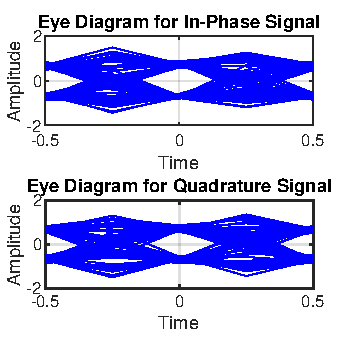
\includegraphics[ width=1\textwidth]
			{./sdf/m_qam_system/figures/experimental/results/DSP_homodyne/5noEDFA_16_homodyne_16_6_eye.pdf}
			\label{fig:16GBdSpecMF}
		\end{minipage}
		\begin{minipage}{0.30\textwidth}
			\centering
			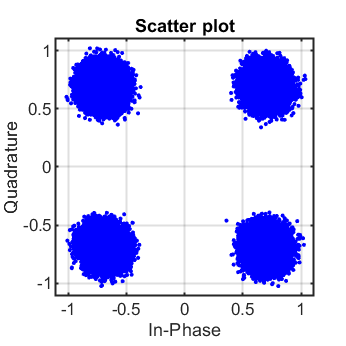
\includegraphics[width=1\textwidth]
			{./sdf/m_qam_system/figures/experimental/results/DSP_homodyne/5noEDFA_16_homodyne_16_6_const.pdf}\\
			\label{fig:16GBdSpecBefFec}
		\end{minipage}
		\caption{Spectrum, eye diagram and constellation after an adaptive equalizer.}
		\label{fig:16GBdFinalHm}
	\end{figure}


	\begin{figure}[H]
		\centering
		\begin{minipage}{0.45\textwidth}
			\centering
			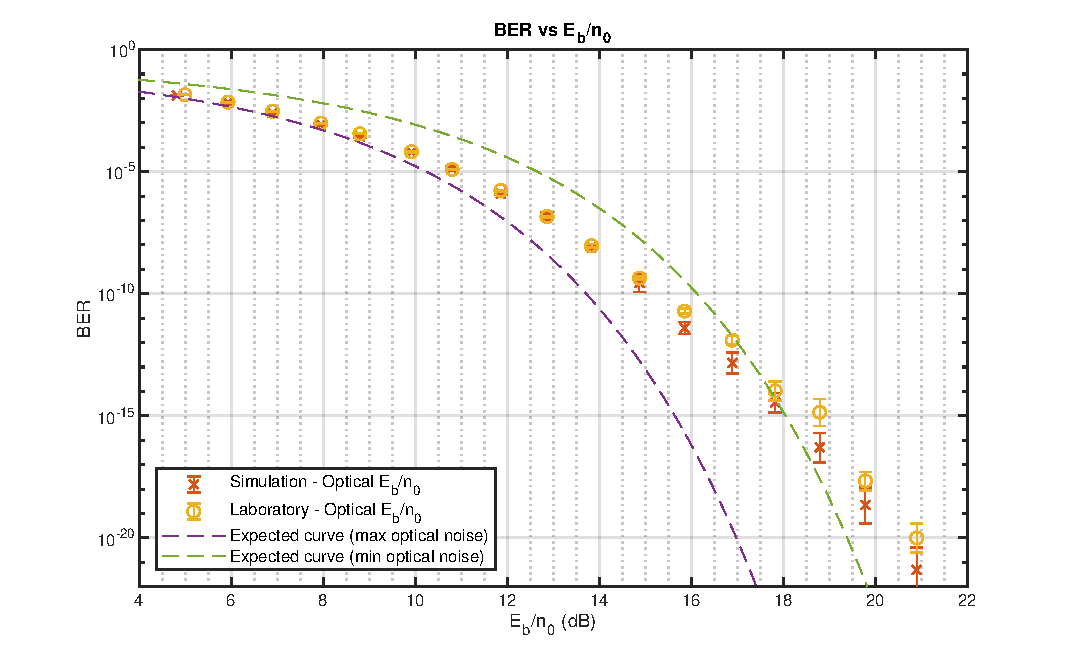
\includegraphics[width=1\textwidth]
			{./sdf/m_qam_system/figures/experimental/results/16GBd_noEDFA/ebn0Curve_sim16_final.pdf}
			\subcaption{\label{fig:16GBdBERH}}
		\end{minipage}
		\begin{minipage}{0.45\textwidth}
			\centering
			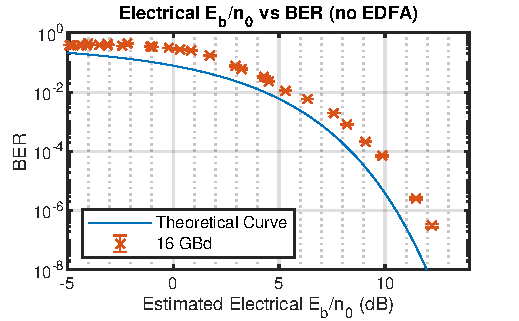
\includegraphics[width=1\textwidth]
			{./sdf/m_qam_system/figures/experimental/results/16GBd_noEDFA/ebn0Curve_lab16_noEDFA_181204.pdf}
			\subcaption{\label{fig:16GBdBERHnoEDFA}}
		\end{minipage}
		\caption{Comparison of expected BER, results from the simulation and from
			the lab setup, plotted against the $E_b/n_0$ measured in the optical
			domain, as described in Sections~\ref{sec:simulValues} and
		\ref{sec:expValues}.\label{fig:16expBerH}}
	\end{figure}

	Two things can be noticed right away from the plot above: the results from the
	simulation are very close to the results from the experimental setup; and
	there are points outside the curves.
	The curves shown were the ones described in Section \ref{sec:simulValues},
	and should coincide with the two simulation points with the highest and lowest $E_b/n_0$.
	Through further testing in the simulation, it was found that the divergence
	from the curves, at leas of the simulated points, is due to the roll-off
	values used. Using a higher roll-off (0.9 instead of 0.05) in the simulation
	made the points follow the curves exactly. However, as the simulations were done
	trying to replicate the conditions of the experimental setup, the values used
	were the same, which led to these results. The same effect can be observed for
	the other symbol rates, with a lower shift from the theoretical curves.

	\subsubsection{4 GBd Signal}


	This section is fairly similar as the one for the 16 GBd signal with homodyne
	receiver.


	Figures~\ref{fig:4GBdinitHmi} to~\ref{fig:4GBdFinalHmi} show the eye diagrams
	and the spectrum of the signals at every stage of the DSP process. The process
	is similar to the described for the 16 GBd signal with homodyne receiver.
	However, some differences can be seen, particularly on the signal spectrum
	before the corrections. However, it can be seen that the distribution of
	points in the final constellation is not optimal, unlike in the 16~GBd case.


	\begin{figure}[H]
		\centering
		\begin{minipage}{0.3\textwidth}
			\centering
			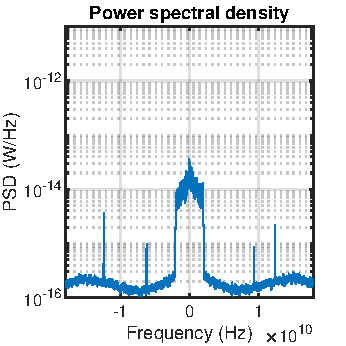
\includegraphics[width=1\textwidth]
			{./sdf/m_qam_system/figures/experimental/results/DSP_homodyne/0noEDFA_4_homodyne_28_4_spectrum.pdf}\\
			\label{fig:16GBdEyeBefFecHm}
		\end{minipage}
		\begin{minipage}{0.3\textwidth}
			\centering
			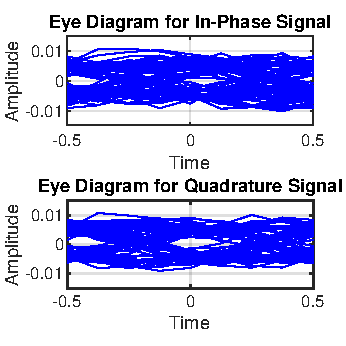
\includegraphics[width=1\textwidth]
			{./sdf/m_qam_system/figures/experimental/results/DSP_homodyne/0noEDFA_4_homodyne_28_4_eye.pdf}
			\label{fig:16GBdSpecBefFecHm}
		\end{minipage}
		\begin{minipage}{0.3\textwidth}
			\centering
			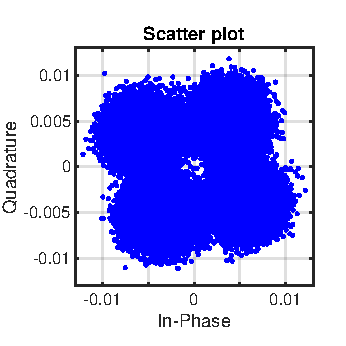
\includegraphics[width=1\textwidth]
			{./sdf/m_qam_system/figures/experimental/results/DSP_homodyne/0noEDFA_4_homodyne_28_4_const.pdf}\\
			\label{fig:16GBdSpecBefFecCHm}
		\end{minipage}
		\caption{Initial spectrum, eye Diagram, and constellation of the original
			signal obtained at the oscilloscope. Input signal power immediately before the
		coherent receiver was -28.4 dBm.}
		\label{fig:4GBdinitHmi}
	\end{figure}


	\begin{figure}[H]
		\centering
		\begin{minipage}{0.30\textwidth}
			\centering
			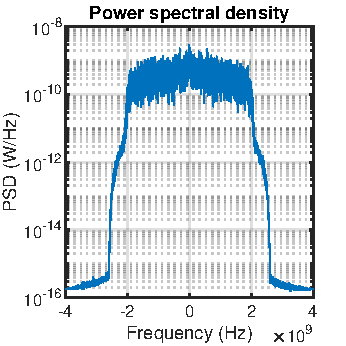
\includegraphics[ width=1\textwidth]
			{./sdf/m_qam_system/figures/experimental/results/DSP_homodyne/2noEDFA_4_homodyne_28_4_spectrum.pdf}\\
			\label{fig:16GBdEyeMf}
		\end{minipage}
		\begin{minipage}{0.30\textwidth}
			\centering
			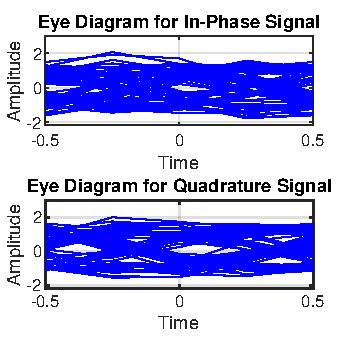
\includegraphics[ width=1\textwidth]
			{./sdf/m_qam_system/figures/experimental/results/DSP_homodyne/2noEDFA_4_homodyne_28_4_eye.pdf}
			\label{fig:16GBdSpecMF}
		\end{minipage}
		\begin{minipage}{0.30\textwidth}
			\centering
			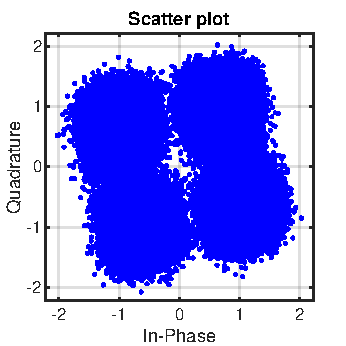
\includegraphics[width=1\textwidth]
			{./sdf/m_qam_system/figures/experimental/results/DSP_homodyne/2noEDFA_4_homodyne_28_4_const.pdf}\\
			\label{fig:16GBdSpecBefFec}
		\end{minipage}
		\caption{Spectrum, eye-diagram and constellation after applying front-end corrections, matched filtering and resampling to $2 S_R$.}
		\label{fig:16GBMFHm}
	\end{figure}


	\begin{figure}[H]
		\centering
		\begin{minipage}{0.30\textwidth}
			\centering
			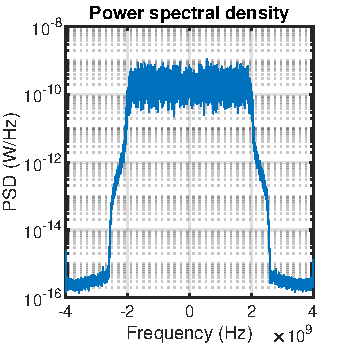
\includegraphics[ width=1\textwidth]
			{./sdf/m_qam_system/figures/experimental/results/DSP_homodyne/3noEDFA_4_homodyne_28_4_spectrum.pdf}\\
			\label{fig:16GBdEyeMf}
		\end{minipage}
		\begin{minipage}{0.30\textwidth}
			\centering
			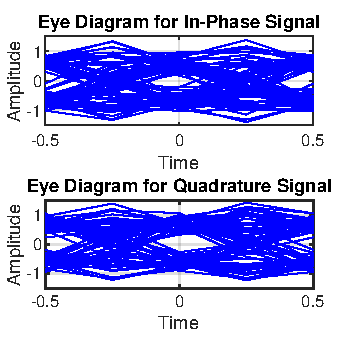
\includegraphics[ width=1\textwidth]
			{./sdf/m_qam_system/figures/experimental/results/DSP_homodyne/3noEDFA_4_homodyne_28_4_eye.pdf}
			\label{fig:16GBdSpecMF}
		\end{minipage}
		\begin{minipage}{0.30\textwidth}
			\centering
			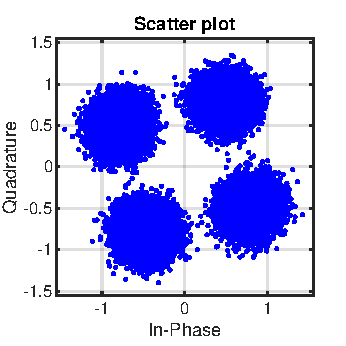
\includegraphics[width=1\textwidth]
			{./sdf/m_qam_system/figures/experimental/results/DSP_homodyne/3noEDFA_4_homodyne_28_4_const.pdf}\\
			\label{fig:16GBdSpecBefFec}
		\end{minipage}
		\caption{Spectrum, eye diagram and constellation after using a contant modulus
		algorithm.}
		\label{fig:16GBMFHm}
	\end{figure}


	\begin{figure}[H]
		\centering
		\begin{minipage}{0.30\textwidth}
			\centering
			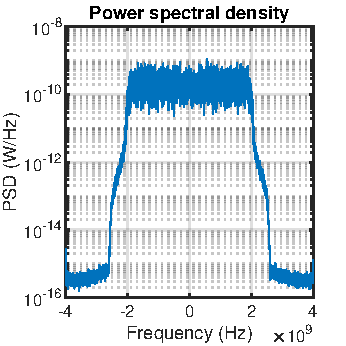
\includegraphics[ width=1\textwidth]
			{./sdf/m_qam_system/figures/experimental/results/DSP_homodyne/4noEDFA_4_homodyne_28_4_spectrum.pdf}\\
			\label{fig:16GBdEyeMf}
		\end{minipage}
		\begin{minipage}{0.30\textwidth}
			\centering
			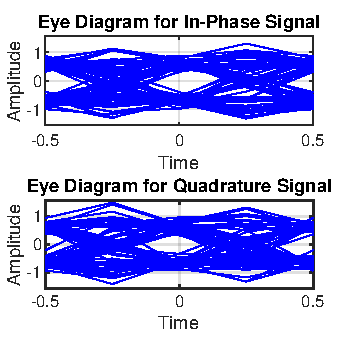
\includegraphics[ width=1\textwidth]
			{./sdf/m_qam_system/figures/experimental/results/DSP_homodyne/4noEDFA_4_homodyne_28_4_eye.pdf}
			\label{fig:16GBdSpecMF}
		\end{minipage}
		\begin{minipage}{0.30\textwidth}
			\centering
			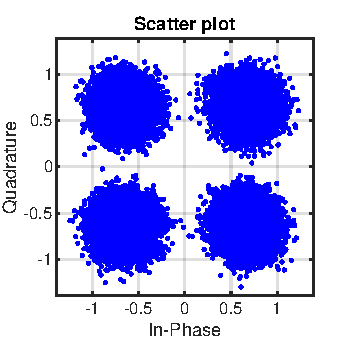
\includegraphics[width=1\textwidth]
			{./sdf/m_qam_system/figures/experimental/results/DSP_homodyne/4noEDFA_4_homodyne_28_4_const.pdf}\\
			\label{fig:16GBdSpecBefFec}
		\end{minipage}
		\caption{Spectrum, eye diagram and constellation after carrier-phase
		compensation.}
		\label{fig:16GBMFHm}
	\end{figure}


	\begin{figure}[H]
		\centering
		\begin{minipage}{0.30\textwidth}
			\centering
			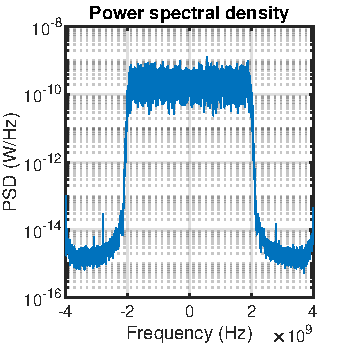
\includegraphics[ width=1\textwidth]
			{./sdf/m_qam_system/figures/experimental/results/DSP_homodyne/5noEDFA_4_homodyne_28_4_spectrum.pdf}\\
			\label{fig:16GBdEyeMf}
		\end{minipage}
		\begin{minipage}{0.30\textwidth}
			\centering
			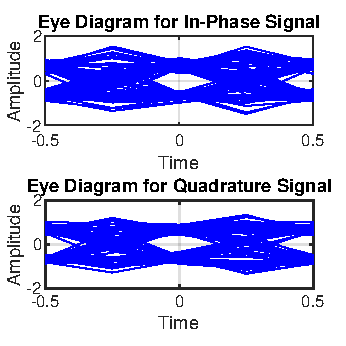
\includegraphics[ width=1\textwidth]
			{./sdf/m_qam_system/figures/experimental/results/DSP_homodyne/5noEDFA_4_homodyne_28_4_eye.pdf}
			\label{fig:16GBdSpecMF}
		\end{minipage}
		\begin{minipage}{0.30\textwidth}
			\centering
			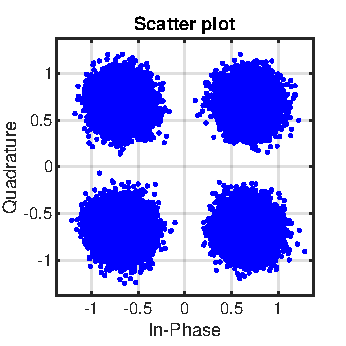
\includegraphics[width=1\textwidth]
			{./sdf/m_qam_system/figures/experimental/results/DSP_homodyne/5noEDFA_4_homodyne_28_4_const.pdf}\\
			\label{fig:16GBdSpecBefFec}
		\end{minipage}
		\caption{Spectrum, eye diagram and constellation after an adaptive equalizer.}
		\label{fig:4GBdFinalHmi}
	\end{figure}


	\begin{figure}[H]
		\centering
		\begin{minipage}{0.45\textwidth}
			\centering
			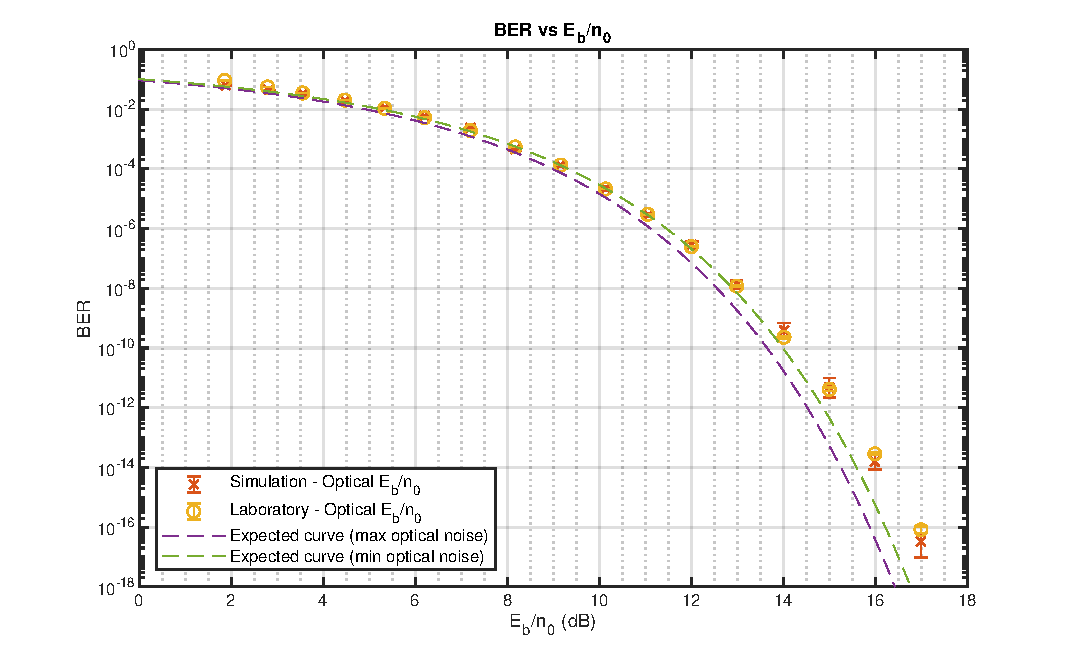
\includegraphics[width=1\textwidth]
			{./sdf/m_qam_system/figures/experimental/results/4GBd_noEDFA/ebn0Curve_sim4_final.pdf}
			\subcaption{\label{fig:4GBdBERH}}
		\end{minipage}
		\begin{minipage}{0.45\textwidth}
			\centering
			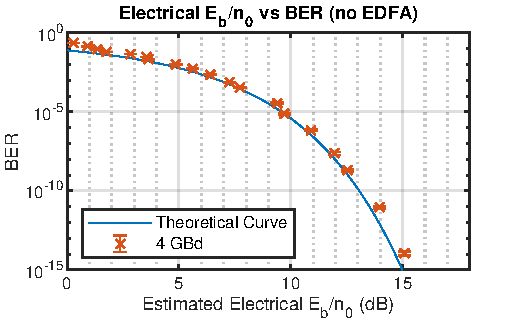
\includegraphics[width=1\textwidth]
			{./sdf/m_qam_system/figures/experimental/results/4GBd_noEDFA/ebn0Curve_lab4_noEDFA_181204.pdf}
			\subcaption{\label{fig:4GBdBERHnoEDFA}}
		\end{minipage}
		\caption{Comparison of expected BER, results from the simulation and from
			the lab setup, plotted against the $E_b/n_0$ measured in the optical
			domain, as described in Sections~\ref{sec:simulValues} and
		\ref{sec:expValues}.\label{fig:4GBdBERH2}}
	\end{figure}

	This plot is pretty similar to the 16 GBd. The major difference here is that
	the two curves appear to be much closer together. As the curves depend on the
	relation between optical and electrical noise, this is to be expected. In this
	case, the transmitter power was typically much lower than in the 16 GBd plot,
	and it was spread through a smaller range. This means that the variation on
	the optical noise produced by the EDFA wasn't as noticeable, and therefore the
	curves should be closer together.

	\subsubsection{1.25 GBd signal}

	This section is similar as the one for the 16GBd signal with homodyne receiver.

	Figures~\ref{fig:1250MBdinitHmi} to~\ref{fig:1250MBdFinalHmi} show the eye diagrams and the spectrum of the signals at every stage of the DSP process. The process is similar to the described for the 16 GBd signal with homodyne receiver. However, some differences can be seen, particularly on the signal spectrum before the corrections. However, it can be seen that the distribution of points in the final constellation is not optimal, unlike in the 16~GBd case.

	\begin{figure}[H]
		\centering
		\begin{minipage}{0.3\textwidth}
			\centering
			\includegraphics[width=1\textwidth]
			{./sdf/m_qam_system/figures/experimental/results/DSP_homodyne/0noEDFA_1_25_homodyne_22_2_spectrum.pdf}\\
			\label{fig:1250MBdEyeBefFecHm}
		\end{minipage}
		\begin{minipage}{0.3\textwidth}
			\centering
			\includegraphics[width=1\textwidth]
			{./sdf/m_qam_system/figures/experimental/results/DSP_homodyne/0noEDFA_1_25_homodyne_22_2_eye.pdf}
			\label{fig:1250MBdSpecBefFecHm}
		\end{minipage}
		\begin{minipage}{0.3\textwidth}
			\centering
			\includegraphics[width=1\textwidth]
			{./sdf/m_qam_system/figures/experimental/results/DSP_homodyne/0noEDFA_1_25_homodyne_22_2_const.pdf}\\
			\label{fig:1250MBdSpecBefFecCHm}
		\end{minipage}
		\caption{Initial spectrum, eye Diagram, and constellation of the original
			signal obtained at the oscilloscope. Input signal power immediately before the
		coherent receiver was -22.2 dBm.}
		\label{fig:1250MBdinitHmi}
	\end{figure}


	\begin{figure}[H]
		\centering
		\begin{minipage}{0.30\textwidth}
			\centering
			\includegraphics[ width=1\textwidth]
			{./sdf/m_qam_system/figures/experimental/results/DSP_homodyne/2noEDFA_1_25_homodyne_22_2_spectrum.pdf}\\
			\label{fig:1250MBdEyeMf}
		\end{minipage}
		\begin{minipage}{0.30\textwidth}
			\centering
			\includegraphics[ width=1\textwidth]
			{./sdf/m_qam_system/figures/experimental/results/DSP_homodyne/2noEDFA_1_25_homodyne_22_2_eye.pdf}
			\label{fig:1250MBdSpecMF}
		\end{minipage}
		\begin{minipage}{0.30\textwidth}
			\centering
			\includegraphics[width=1\textwidth]
			{./sdf/m_qam_system/figures/experimental/results/DSP_homodyne/2noEDFA_1_25_homodyne_22_2_const.pdf}\\
			\label{fig:1250MBdSpecBefFec}
		\end{minipage}
		\caption{Spectrum, eye-diagram and constellation after applying front-end corrections, matched filtering and resampling to $2 S_R$.}
		\label{fig:1250MBMFHm}
	\end{figure}


	\begin{figure}[H]
		\centering
		\begin{minipage}{0.30\textwidth}
			\centering
			\includegraphics[ width=1\textwidth]
			{./sdf/m_qam_system/figures/experimental/results/DSP_homodyne/3noEDFA_1_25_homodyne_22_2_spectrum.pdf}\\
			\label{fig:1250MBdEyeMf}
		\end{minipage}
		\begin{minipage}{0.30\textwidth}
			\centering
			\includegraphics[ width=1\textwidth]
			{./sdf/m_qam_system/figures/experimental/results/DSP_homodyne/3noEDFA_1_25_homodyne_22_2_eye.pdf}
			\label{fig:1250MBdSpecMF}
		\end{minipage}
		\begin{minipage}{0.30\textwidth}
			\centering
			\includegraphics[width=1\textwidth]
			{./sdf/m_qam_system/figures/experimental/results/DSP_homodyne/3noEDFA_1_25_homodyne_22_2_const.pdf}\\
			\label{fig:1250MBdSpecBefFec}
		\end{minipage}
		\caption{Spectrum, eye diagram and constellation after using a constant modulus
		algorithm.}
		\label{fig:1250MBMFHm}
	\end{figure}


	\begin{figure}[H]
		\centering
		\begin{minipage}{0.30\textwidth}
			\centering
			\includegraphics[ width=1\textwidth]
			{./sdf/m_qam_system/figures/experimental/results/DSP_homodyne/4noEDFA_1_25_homodyne_22_2_spectrum.pdf}\\
			\label{fig:1250MBdEyeMf}
		\end{minipage}
		\begin{minipage}{0.30\textwidth}
			\centering
			\includegraphics[ width=1\textwidth]
			{./sdf/m_qam_system/figures/experimental/results/DSP_homodyne/4noEDFA_1_25_homodyne_22_2_eye.pdf}
			\label{fig:1250MBdSpecMF}
		\end{minipage}
		\begin{minipage}{0.30\textwidth}
			\centering
			\includegraphics[width=1\textwidth]
			{./sdf/m_qam_system/figures/experimental/results/DSP_homodyne/4noEDFA_1_25_homodyne_22_2_const.pdf}\\
			\label{fig:1250MBdSpecBefFec}
		\end{minipage}
		\caption{Spectrum, eye diagram and constellation after carrier-phase
		compensation.}
		\label{fig:1250MBMFHm}
	\end{figure}


	\begin{figure}[H]
		\centering
		\begin{minipage}{0.30\textwidth}
			\centering
			\includegraphics[ width=1\textwidth]
			{./sdf/m_qam_system/figures/experimental/results/DSP_homodyne/5noEDFA_1_25_homodyne_22_2_spectrum.pdf}\\
			\label{fig:1250MBdEyeMf}
		\end{minipage}
		\begin{minipage}{0.30\textwidth}  
			\centering
			\includegraphics[clip, trim=0cm 0cm 0cm 0cm, width=1\textwidth]
			{./sdf/m_qam_system/figures/experimental/results/DSP_homodyne/5noEDFA_1_25_homodyne_22_2_eye.pdf}
			\label{fig:1250MBdSpecMF}
		\end{minipage}
		\begin{minipage}{0.30\textwidth}
			\centering
			\includegraphics[width=1\textwidth]
			{./sdf/m_qam_system/figures/experimental/results/DSP_homodyne/5noEDFA_1_25_homodyne_22_2_const.pdf}\\
			\label{fig:1250MBdSpecBefFec}
		\end{minipage}
		\caption{Spectrum, eye diagram and final constellation after an adaptive
		equalizer. The BER estimated from the Q-factor is $9.2598 \times 10^{-29}$}
		\label{fig:1250MBdFinalHmi}
	\end{figure}

	\begin{figure}[H]
		\centering
		\begin{minipage}{0.45\textwidth}
			\centering
			\includegraphics[width=1\textwidth]
			{./sdf/m_qam_system/figures/experimental/results/1_25GBd_noEDFA/ebn0Curve_sim1_25_final.pdf}
			\subcaption{\label{fig:1.25GBdBERH}}
		\end{minipage}
		\begin{minipage}{0.45\textwidth}
			\centering
			\includegraphics[width=1\textwidth]
			{./sdf/m_qam_system/figures/experimental/results/1_25GBd_noEDFA/ebn0Curve_lab1_25_noEDFA_181204.pdf}
			\subcaption{\label{fig:1.25GBdBERHnoEDFA}}
		\end{minipage}
		\caption{Comparison of expected BER, results from the simulation and from
			the lab setup, plotted against the $E_b/n_0$ measured in the optical
			domain, as described in Sections~\ref{sec:simulValues} and
		\ref{sec:expValues}.\label{fig:4GBdBERH2}}
	\end{figure}

	This plot is not very different from the 4 GBd case, and the simulation
	continues to show good agreement with the experimental results.




% vim: set ts=2 sw=2 tw=80 noet :
